\documentclass[11pt]{exam}

\newcommand{\Version}{6} 
\newcommand{\Solutions}{1} 
\newcommand{\Set}{1} % can set to any integer initially

% TEST SPECIFIC INFORMATION
\ifnum \Version=1 \newcommand{\TestName}{Final Exam} \fi
\ifnum \Version=2 \newcommand{\TestName}{Final Exam  Version A} \fi
\ifnum \Version=3 \newcommand{\TestName}{Final Exam  Version B} \fi
\ifnum \Version=4 \newcommand{\TestName}{Final Exam  Version C} \fi
% 2024
\ifnum \Version=5 \newcommand{\TestName}{Final Exam Make-up A} \fi
\ifnum \Version=6 \newcommand{\TestName}{Final Exam  Version A} \fi
\ifnum \Version=7 \newcommand{\TestName}{Final Exam  Version B} \fi

% LOAD PACKAGES
\usepackage{amsmath} % allows for align env and other things
\usepackage{amssymb} % 
\usepackage{mathtools} % allows for single apostrophe
\usepackage{enumitem} % allows for alpha lettering in enumerated lists
\usepackage{lastpage}
\usepackage{array} % for table alignments

\usepackage{graphicx} % if images are needed
\usepackage{wrapfig} % to allow text wrapping

\addpoints

\usepackage{pgfplots} % for surfaces (chapter 7)
\usepackage{tikz-3dplot} 
\pgfplotsset{compat=1.9}
\usetikzlibrary{decorations.pathmorphing,patterns} % for some tikz diagrams
% ~~~~~~~~~~~~~~~~~~~~~~~~~~~~~~~~~~~~
% INITIALS
\newcommand{\Initials}{\textit{\Course, \TestName. Your initials: \underline{\hspace{3cm}}} \vspace{1pt}}

\newcommand{\InitialsLeft}{\noindent \hspace{-18pt}\textit{\Course, \TestName. Your initials: \underline{\hspace{3cm}}} \vspace{1pt}}

\newcommand{\InitialsRight}{\begin{flushright}\textit{\Course, \TestName. Your initials: \underline{\hspace{3cm}}} \vspace{1pt}\end{flushright}}

% ADJUST FIRST LINE IN PARAGRAPH INDENTATION 
\setlength\parindent{0pt}

% FONT FORMAT
\renewcommand*\rmdefault{lmss} % change font to lat mod ss

% ADJUST MARGINS 
\usepackage[a4paper, tmargin=0.8in,bmargin=0.8in,left=1in,right=1in]{geometry}

% TIKZ DIAGRAMS
\usepackage{color}
\usepackage{tikz}  \usetikzlibrary{arrows} 
\usetikzlibrary{calc} 

% COURSE SPECIFIC INFORMATION
\newcommand{\Course}{Math 2552, Differential Equations}
\newcommand{\Instructors}{}

\newcommand{\LastPage}{\begin{center}\textit{This page may be used for scratch work. Please indicate clearly if you would like your work on this page to be graded. }\end{center}   }

% DERIVATIVES
\newcommand{\dfdy}{{\frac{df}{dy}}} % 
\newcommand{\dydt}{{\frac{dy}{dt}}} % 
\newcommand{\dxdt}{{\frac{dx}{dt}}} % 
\newcommand{\dydx}{{\frac{dy}{dx}}} % 
\newcommand{\dydtt}{{\frac{d ^2y}{dt^2}}} % 
\newcommand{\dydxx}{{\frac{d^2y}{dx^2}}} % 
\newcommand{\dydttt}{{\frac{d^3y}{dt^3}}} % 

\newcommand{\ddt}{{\frac{d}{dt}}} % 
\newcommand{\ddx}{{\frac{d}{dx}}} % 
\newcommand{\ddy}{{\frac{d}{dy}}} % 
\newcommand{\dudt}{{\frac{du}{dt}}} % 
\newcommand{\dvdx}{{\frac{dv}{dx}}} % 
\newcommand{\dxdtt}{{\frac{d^2x}{dt^2}}} % 
\newcommand{\dzdt}{{\frac{dz}{dt}}} % 

% COLORS FOR SOLUTIONS
\definecolor{DarkBlue}{rgb}{0.0,0.2,0.4} % 
\definecolor{DarkRed}{rgb}{0.4,0.1,0.1} % 
\definecolor{DarkGreen}{rgb}{0.0,0.25,0.15} % 
\newcommand*{\TickSize}{4pt}%

\newcommand*{\AxisMin}{0}%
\newcommand*{\AxisMax}{0}%

\newcommand*{\DrawHorizontalPhaseLine}[4][]{%
    % #1 = axis tick labels
    % #2 = right arrows positions as CSV
    % #3 = left arrow positions as CSV
    \gdef\AxisMin{0}%
    \gdef\AxisMax{0}%
    \edef\MyList{#2}% Allows for #1 to be both a macro or not
    \foreach \X in \MyList {
        \draw  (\X,\TickSize) -- (\X,-\TickSize) node [below] {$\X$};
        \ifnum\AxisMin>\X
            \xdef\AxisMin{\X}%
        \fi
        \ifnum\AxisMax<\X
            \xdef\AxisMax{\X}%
        \fi
    }

    \edef\MyList{#3}% Allows for #2 to be both a macro or not
    \foreach \X in \MyList {% Right arrows
        \draw [->] (\X-0.1,0) -- (\X,0);
        \ifnum\AxisMin>\X
            \xdef\AxisMin{\X}%
        \fi
        \ifnum\AxisMax<\X
            \xdef\AxisMax{\X}%
        \fi
    }

    \edef\MyList{#4}% Allows for #3 to be both a macro or not
    \foreach \X in \MyList {% Left arrows
        \draw [<-] (\X-0.1,0) -- (\X,0);
        \ifnum\AxisMin>\X
            \xdef\AxisMin{\X}%
        \fi
        \ifnum\AxisMax<\X
            \xdef\AxisMax{\X}%
        \fi
    }

    \draw  (\AxisMin-1,0) -- (\AxisMax+1,0) node [right] {#1};
}%

\newcommand*{\DrawVerticalPhaseLine}[4][]{%
    % #1 = axis tick labels
    % #2 = up arrows positions as CSV
    % #3 = down arrow positions as CSV
    \gdef\AxisMin{0}%
    \gdef\AxisMax{0}%
    \edef\MyList{#2}% Allows for #1 to be both a macro or not
    \foreach \X in \MyList {
        \draw  (-\TickSize,\X) -- (\TickSize,\X) node [right] {$\X$};
        \ifnum\AxisMin>\X
            \xdef\AxisMin{\X}%
        \fi
        \ifnum\AxisMax<\X
            \xdef\AxisMax{\X}%
        \fi
    }

    \edef\MyList{#3}% Allows for #2 to be both a macro or not
    \foreach \X in \MyList {% Up arrows
        \draw [->] (0,\X-0.1) -- (0,\X);
        \ifnum\AxisMin>\X
            \xdef\AxisMin{\X}%
        \fi
        \ifnum\AxisMax<\X
            \xdef\AxisMax{\X}%
        \fi
    }

    \edef\MyList{#4}% Allows for #3 to be both a macro or not
    \foreach \X in \MyList {% Down arrows
        \draw [->] (0,\X+0.1) -- (0,\X);
        \ifnum\AxisMin>\X
            \xdef\AxisMin{\X}%
        \fi
        \ifnum\AxisMax<\X
            \xdef\AxisMax{\X}%
        \fi
    }

    \draw  (0,\AxisMin-1) -- (0,\AxisMax+1) node [above] {#1};
}%

% HEADERS AND FOOTERS
\pagestyle{headandfoot}
% \runningfooter{}{}{}
\runningfooter{}{}{\textit{Page \thepage \ of \pageref{LastPage}} }
\runningheader{\textit{Please write your last name: \framebox{\strut\hspace{5cm}} }}{}{\textit{\TestName} }

% ~~~ ~~~ ~~~ ~~~ ~~~ ~~~ ~~~ ~~~ ~~~ ~~~ ~~~ ~~~ ~~~ ~~~
\begin{document}

% REDUCE VERSIONS FOR SANITY
\ifnum \Version=5
    \renewcommand{\Version}{4}
\fi

% SCRAMBLE QUESTION ORDER
\ifnum \Version=1
    \renewcommand{\Set}{1}
\fi
\ifnum \Version=2
    \renewcommand{\Set}{2}
\fi
\ifnum \Version=3
    \renewcommand{\Set}{3}
\fi
\ifnum \Version=4
    \renewcommand{\Set}{4}
\fi
\ifnum \Version>5
    \renewcommand{\Set}{5}
\fi

\vspace*{-1cm}

% TITLE 
\begin{center}
\ifnum \Solutions=1 {\Large {\color{DarkBlue}\textit{\TestName \ Solutions}}\\[4pt]}
\else 
    {\Large \TestName, \Course}
\fi
\end{center}

% NAME AND STUDENT ID
\newcommand{\ID}{Please enter the remaining digits of your GTID:  \framebox{\strut $9$}\framebox{\strut $0$}\framebox{\strut\hspace{0.19cm}}\framebox{\strut\hspace{0.19cm}}\framebox{\strut\hspace{0.19cm}}\framebox{\strut\hspace{0.19cm}}\framebox{\strut\hspace{0.19cm}}\framebox{\strut\hspace{0.19cm}}\framebox{\strut\hspace{0.19cm}}, and with all CAPITAL LETTERS  print your first name: \framebox{\strut\hspace{3.6cm}}, and last name: \framebox{\strut\hspace{3.8cm}}.}
\ID

% FORMULA SHEET
\begin{center}
    \textbf{First Order Systems}\\
        2D Repeated eigenvalues: $\displaystyle (A-\lambda I) \vec w = \vec v, \quad \vec w = t\vec v + \vec c $
        
        \textbf{Complex Eigenvalues}\\
        $\displaystyle 
        \lambda_k = \alpha + i \beta, \ \beta \ne 0 , \ \vec v_k = \vec a + i \vec b, \ 
        \vec x_k = e^{\alpha t} (\vec a \cos \beta t - \vec b \sin \beta t), 
        \ 
        \vec x_{k+1} = e^{\alpha t} (\vec a \sin \beta t + \vec b \cos \beta t) $

    \vspace{0pt}
    \textbf{Second Order Homogeneous Constant Coefficient}
    \begin{tabular}{ p{4.2cm} p{4.6cm} }
        
        $\lambda_1, \lambda_2$ &  general solution 
        \\[2pt] \hline 
        real distinct &  $c_1 e^{\lambda_1 t} + c_2 e^{\lambda_2 t}$\\       
        real repeated, $\lambda_1 = \lambda_2$ & $c_1 e^{\lambda_1 t} + c_2 t e^{\lambda_1 t}$\\
        complex, $\lambda_1 = \alpha + i \beta$ & $e^{\alpha t} \left( c_1 \cos \beta t + c_2 \sin \beta t \right)$\\[2pt] \hline
    \end{tabular}    
    
    \vspace{4pt}
    \textbf{Second Order Homogeneous Cauchy-Euler}
    \begin{tabular}{ p{6.2cm} p{6cm} }
        roots &  general solution 
        \\[2pt] \hline 
        real distinct, $m_1 \ne m_2$ &  $c_1 t^{m_1} + c_2 t^{m_2}$\\       
        real repeated, $m = m_1 = m_2$ & $c_1 t^{m} + c_2 t^m \ln(t)$\\
        complex, $m_1 = \alpha + i \beta$ & $c_1t^{\alpha}\cos(\beta \ln(t)) + c_2t^{\alpha}\sin(\beta \ln (t))$\\[2pt] \hline
    \end{tabular}
    
    \vspace{4pt}
    
    \textbf{Undetermined Coefficients} 
        \vspace{-6pt}
    \begin{align*}
        P_n &= a_0t^n + a_1t^{n-1} \ldots + a_n, \
        Q_n = A_0t^n + A_1t^{n-1} \ldots + A_n, \       
        R_n = B_0t^n + B_1t^{n-1} \ldots + B_n     
    \end{align*}\vspace{-0.4cm}\setlength{\extrarowheight}{0.05cm}
    \begin{tabular}{ p{3.9cm} p{5cm} }
        $g(t)$ &  particular solution $y_p(t)$ 
        \\[2pt] \hline $P_n(t)$  & $t^s Q_n$   \\        
        $P_n(t)e^{\alpha t}$ &  $t^s e^{\alpha t}Q_n$\\       
        $P_n(t)e^{\alpha t}\sin(\beta t)$ & $t^s e^{\alpha t} \left(\cos(\beta t)Q_n+\sin(\beta t) R_n\right)$\\
        $P_n(t)e^{\alpha t}\cos(\beta t)$ & $t^s e^{\alpha t} \left(\cos(\beta t)Q_n+\sin(\beta t) R_n\right)$\\[2pt] \hline
    \end{tabular}
    \setlength{\extrarowheight}{0.0cm}

    \vspace{15pt}
    \textbf{Variation of Parameters}    
        \vspace{-0.2cm}
    \begin{align*}
        \text{scalar form: } y_p &= v_1 (t) y_1(t) + v_2(t) y_2(t) , \quad 
        v_1 = - \int \frac{y_2(t)g(t)}{W[y_1,y_2]}dt , \quad 
        v_2 = \int \frac{y_1(t)g(t)}{W[y_1,y_2]} dt \\
        \text{first-order system: }\vec x \, ' &= P \vec x + \vec g(t), \quad \vec x_p = X(t) \int X^{-1}(t) \vec g(t) \, dt \\
         \text{matrix inverse: if } A &= \begin{pmatrix} a& b\\c&d\end{pmatrix}, \ \text{then } A^{-1} = \frac{1}{|A|}\begin{pmatrix} d&-b\\-c&a\end{pmatrix}
    \end{align*}        
    
\end{center}


\def\dm{\displaystyle}

\begin{center}
    {\bf Laplace Transforms}\\[1pt]
\end{center}
$
\hspace*{-.5em}
\begin{array}{lllllll}
 1.  & 1 \quad  & 1/s,\quad s>0 & \qquad  \ \quad & 10.  & t^n e^{at}\  \quad  & \frac{n!}{(s-a)^{n+1}},\quad s>a\\[0ex] 
 2.  & e^{at} \quad  & 1/(s-a),\quad s>a  & \qquad  \ \quad & 11. & u_c(t)\ \ (c\ge 0) \quad  & e^{-cs}/s,\quad s>0 \\[0ex]
 3.  & t^n  \quad  & n!/s^{n+1},\quad s>0 & \qquad  \ \quad & 12.  & u_c(t)f(t-c)\  \quad  & \dm e^{-cs} F(s), \ c\ge 0 \\[0ex] 
 4.  & \sin(at) \quad  & a/(s^2+a^2),\quad s>0  & \qquad  \ \quad & 13.  & e^{ct}f(t) \quad  & \dm F(s-c) \\[0ex] 
 5.  & \cos(at) \quad  & s/(s^2+a^2),\quad s>0  & \qquad  \ \quad & 14.  & t^n f(t) \quad  & \dm (-1)^n F^{(n)}(s) \\[0ex]
 6.  & e^{at}\sin(bt) \quad  & \dm\frac{b}{(s-a)^2+b^2},\quad s>a  & \qquad  \ \quad & 15. & f(t-T) = f(t) \quad  & \dm \frac{1}{1-e^{-sT}}\int_0^Te^{-st}f(t)\,dt \\[0ex]
 7.  & e^{at}\cos(bt) \quad  & \dm\frac{s-a}{(s-a)^2+b^2},\quad s>a & \qquad  \ \quad &  16. & \delta(t-c) & e^{-cs}\\[0ex]
 8.  & f'(t) \  \quad  &  sF(s) - f(0) & \qquad  \ \quad & 17. & f\ast g & F(s)G(s) \\[0ex]
 9.  & f''(t) \  \quad   & s^2F(s) - sf(0) - f'(0) & \qquad  \ \quad &  & & \\[0ex]
\end{array} 
$

\begin{center}
    {\bf Response Functions}\\[0pt]
\end{center}
\setlength{\extrarowheight}{0.05cm}
\begin{center}
\begin{tabular}{ p{2.2cm} p{2.4cm} p{0.2cm} p{4.2cm} p{0.2cm} p{3.3cm} }
    domain &  total response & & Free Response & & Forced Response \\[2pt] \hline 
    $s-$domain & \centering $Y(s)$ & $=$ & $H \cdot \left[ (as+b) y(0) + ay'(0) \right]$ & $+$ & $HG$ \\ 
    $t-$domain & \centering $y(t)$ & $=$ & $c_1y_1 + c_2y_2$ & $+$ & $\int_0^t h(t-\tau) g(\tau) \, d\tau$ \\[2pt] 
    \hline
\end{tabular}
\end{center}
\setlength{\extrarowheight}{0cm}

% EXAM STARTS HERE
\newpage

\begin{questions}

    \ifnum \Set>0

        \ifnum \Version=1
\question[2] You do not need to show your work for this question. Consider the differential equation below.
$$\displaystyle t\, \dydt + 2y^2 = \cos t$$
\begin{parts}
    \part Fill in the appropriate circle to indicate whether the DE is homogeneous or inhomogeneous.
    \begin{itemize}        
        \item[$\bigcirc$] The DE is homogeneous.
        \item[$\bigcirc$] The DE is inhomogeneous.
    \end{itemize}     
    \ifnum \Solutions=1 {\color{DarkBlue} DE is inhomogeneous because of the $\cos t$ term. } \fi
    \part Fill in the appropriate circle to indicate whether the DE is linear or non-linear
    \begin{itemize}
        \item[$\bigcirc$] The DE is linear.
        \item[$\bigcirc$] The DE is non-linear.
    \end{itemize}
    \ifnum \Solutions=1 {\color{DarkBlue} DE is non-linear because of the $y^2$ term. } \fi    
    \part Fill in the appropriate circle to indicate whether the DE is autonomous or not autonomous. 
    \begin{itemize}        
        \item[$\bigcirc$] The DE is autonomous.
        \item[$\bigcirc$] The DE is not autonomous.
    \end{itemize}       
    \ifnum \Solutions=1 {\color{DarkBlue} DE is not autonomous because $t$ appears as a coefficient of the $y'$ term, and also because $t$ appears in the $\cos t$ term. } \fi    
    \part What is the order of the DE? \framebox{\strut\hspace{2cm}}
    \ifnum \Solutions=1 {\color{DarkBlue} \\ The order of the DE is 1 because the highest order derivative is a first order derivative. } \fi    
\end{parts}
\fi 

\ifnum \Version=2
\question[2] You do not need to show your work for this question. Consider the differential equation below.
$$\displaystyle y''' + 2y^2 = 3$$
\begin{parts}
    \part Fill in the appropriate circle to indicate whether the DE is homogeneous or inhomogeneous.
    \begin{itemize}        
        \item[$\bigcirc$] The DE is homogeneous.
        \item[$\bigcirc$] The DE is inhomogeneous.
    \end{itemize}     
    \ifnum \Solutions=1 {\color{DarkBlue} DE is inhomogeneous because of the $3$ term. } \fi
    \part Fill in the appropriate circle to indicate whether the DE is linear or non-linear
    \begin{itemize}
        \item[$\bigcirc$] The DE is linear.
        \item[$\bigcirc$] The DE is non-linear.
    \end{itemize}
    \ifnum \Solutions=1 {\color{DarkBlue} DE is non-linear because of the $y^2$ term. } \fi    
    \part Fill in the appropriate circle to indicate whether the DE is autonomous or not autonomous. 
    \begin{itemize}        
        \item[$\bigcirc$] The DE is autonomous.
        \item[$\bigcirc$] The DE is not autonomous.
    \end{itemize}       
    \ifnum \Solutions=1 {\color{DarkBlue} DE is autonomous because $t$ does not appear in the DE. } \fi    
    \part What is the order of the DE? \framebox{\strut\hspace{2cm}}
    \ifnum \Solutions=1 {\color{DarkBlue} \\ The order of the DE is 3 because the highest order derivative is a third order derivative. } \fi    
\end{parts}
\fi 



\ifnum \Version=3
\question[2] You do not need to show your work for this question. Consider the differential equation below.
$$\displaystyle y'' + 2t^3y = t+1$$
\begin{parts}
    \part Fill in the appropriate circle to indicate whether the DE is homogeneous or inhomogeneous.
    \begin{itemize}        
        \item[$\bigcirc$] The DE is homogeneous.
        \item[$\bigcirc$] The DE is inhomogeneous.
    \end{itemize}     
    \ifnum \Solutions=1 {\color{DarkBlue} DE is inhomogeneous because of the $t+1$ term. } \fi
    \part Fill in the appropriate circle to indicate whether the DE is linear or non-linear
    \begin{itemize}
        \item[$\bigcirc$] The DE is linear.
        \item[$\bigcirc$] The DE is non-linear.
    \end{itemize}
    \ifnum \Solutions=1 {\color{DarkBlue} DE is linear because of the coefficients of $y$ and $y''$ are not functions of $y$. } \fi    
    \part Fill in the appropriate circle to indicate whether the DE is autonomous or not autonomous. 
    \begin{itemize}        
        \item[$\bigcirc$] The DE is autonomous.
        \item[$\bigcirc$] The DE is not autonomous.
    \end{itemize}       
    \ifnum \Solutions=1 {\color{DarkBlue} DE is not autonomous because $t$ appears in the DE. } \fi    
    \part What is the order of the DE? \framebox{\strut\hspace{2cm}}
    \ifnum \Solutions=1 {\color{DarkBlue} \\ The order of the DE is 2 because the highest order derivative is a second order derivative. } \fi    
\end{parts}
\fi 



\ifnum \Version=4
\question[2] You do not need to show your work for this question. Consider the differential equation below.
$$\displaystyle y'' + t^2y' + 2ty = t^4$$
\begin{parts}

    \part Fill in the appropriate circle to indicate whether the DE is linear or non-linear
    \begin{itemize}
        \item[$\bigcirc$] The DE is linear.
        \item[$\bigcirc$] The DE is non-linear.
    \end{itemize}
    \ifnum \Solutions=1 {\color{DarkBlue} DE is linear because of the coefficients of $y$, $y'$, and $y''$ are not functions of $y$. } \fi    
    \part Fill in the appropriate circle to indicate whether the DE is autonomous or not autonomous. 
    \begin{itemize}        
        \item[$\bigcirc$] The DE is autonomous.
        \item[$\bigcirc$] The DE is not autonomous.
    \end{itemize}       
    \ifnum \Solutions=1 {\color{DarkBlue} DE is not autonomous because $t$ appears in the DE. } \fi   
    \part Fill in the appropriate circle to indicate whether the DE is homogeneous or inhomogeneous.
    \begin{itemize}        
        \item[$\bigcirc$] The DE is homogeneous.
        \item[$\bigcirc$] The DE is inhomogeneous.
    \end{itemize}     
    \ifnum \Solutions=1 {\color{DarkBlue} DE is inhomogeneous because of the $t^4$ term. } \fi   
    \part What is the order of the DE? \framebox{\strut\hspace{2cm}}
    \ifnum \Solutions=1 {\color{DarkBlue} \\ The order of the DE is 2 because the highest order derivative is a second order derivative. } \fi    
\end{parts}
\fi 






\ifnum \Version=6
    \question[1] You do not need to show your work for this question. Consider the differential equation below.
    $$\displaystyle y'' + t^2y' + 2ty = 4\cos(t)-\sin(t)$$
    \begin{parts}
    
        \part Fill in the appropriate circle to indicate whether the DE is linear or non-linear
        \begin{itemize}
            \item[$\bigcirc$] The DE is linear.
            \item[$\bigcirc$] The DE is non-linear.
        \end{itemize}
        \ifnum \Solutions=1 {\color{DarkBlue} DE is linear because of the coefficients of $y$, $y'$, and $y''$ are not functions of $y$. } \fi    
        \part Fill in the appropriate circle to indicate whether the DE is autonomous or not autonomous. 
        \begin{itemize}        
            \item[$\bigcirc$] The DE is autonomous.
            \item[$\bigcirc$] The DE is not autonomous.
        \end{itemize}       
        \ifnum \Solutions=1 {\color{DarkBlue} DE is not autonomous because $t$ appears in the DE. } \fi   
        \part Fill in the appropriate circle to indicate whether the DE is homogeneous or inhomogeneous.
        \begin{itemize}        
            \item[$\bigcirc$] The DE is homogeneous.
            \item[$\bigcirc$] The DE is inhomogeneous.
        \end{itemize}     
        \ifnum \Solutions=1 {\color{DarkBlue} DE is inhomogeneous because of the $t^4$ term. } \fi   
        \part What is the order of the DE? \framebox{\strut\hspace{2cm}}
        \ifnum \Solutions=1 {\color{DarkBlue} \\ The order of the DE is 2 because the highest order derivative is a second order derivative. } \fi    
    \end{parts}
\fi 



\ifnum \Version=7
    \question[1] You do not need to show your work for this question. Consider the differential equation below.
    $$\displaystyle y' + 2ty^2 = 4t+1$$
    \begin{parts}
    
        \part Fill in the appropriate circle to indicate whether the DE is linear or non-linear
        \begin{itemize}
            \item[$\bigcirc$] The DE is linear.
            \item[$\bigcirc$] The DE is non-linear.
        \end{itemize}
        \ifnum \Solutions=1 {\color{DarkBlue} DE is non-linear because of the $y^2$ term. } \fi    
        \part Fill in the appropriate circle to indicate whether the DE is autonomous or not autonomous. 
        \begin{itemize}        
            \item[$\bigcirc$] The DE is autonomous.
            \item[$\bigcirc$] The DE is not autonomous.
        \end{itemize}       
        \ifnum \Solutions=1 {\color{DarkBlue} DE is not autonomous because $t$ appears in the DE. } \fi   
        \part Fill in the appropriate circle to indicate whether the DE is homogeneous or inhomogeneous.
        \begin{itemize}        
            \item[$\bigcirc$] The DE is homogeneous.
            \item[$\bigcirc$] The DE is inhomogeneous.
        \end{itemize}     
        \ifnum \Solutions=1 {\color{DarkBlue} DE is inhomogeneous because of the $t^4$ term. } \fi   
        \part What is the order of the DE? \framebox{\strut\hspace{2cm}}
        \ifnum \Solutions=1 {\color{DarkBlue} \\ The order of the DE is 1 because the highest order derivative is a first order derivative. } \fi    
    \end{parts}
\fi

        \ifnum \Version=6
    \question[1] You do not need to show your work for this question. Consider the differential equation $2y'' - 4ty' - 6y = 12$. The DE can be expressed in the form $\vec x\, ' = A\vec x + \vec g$. Fill in the missing entries below to define $A$ and $\vec g$.   
    \begin{align*}
     A = \left( \hbox to 2cm{\vbox to 0.85cm{}} \right), \quad \vec g = \left( \hbox to 1.2cm{\vbox to 0.85cm{}} \right)
    \end{align*}
    
\fi



\ifnum \Version=7
    \question[1] You do not need to show your work for this question. Consider the differential equation $ty'' - 4ty' - 6t^2y = te^{-2t}\cos(2t)$. The DE can be expressed in the form $\vec x\, ' = A\vec x + \vec g$. Fill in the missing entries below to define $A$ and $\vec g$.   
    \begin{align*}
     A = \left( \hbox to 2cm{\vbox to 0.85cm{}} \right), \quad \vec g = \left( \hbox to 1.2cm{\vbox to 0.85cm{}} \right)
    \end{align*}
    \ifnum \Solutions=1 {\color{DarkBlue} 
\textbf{Solutions:}
$$A = \begin{pmatrix} 0&1\\6t&4\end{pmatrix}, \quad g = \begin{pmatrix} 0\\e^{-2t}\cos 2t \end{pmatrix}$$
} 
\else 
\newpage
\fi
\fi
        \ifnum \Version=1  
% Pulled from Test 1 202305
\question[1] Consider the autonomous differential equation $\displaystyle \frac{dy}{dt}= (y-1)(y-k^2)$.  Assume $k$ can be any real number. Draw the bifurcation diagram on the axes below. That is, plot the location of the critical points versus $k$. Please label your axes.


\ifnum \Solutions=1 {\color{DarkBlue} 
        \begin{center}
        \begin{tikzpicture}[scale=0.85]
        \draw[help lines] (-2.5,-2.5) grid (2.5, 2.5);
        \draw[ thick, ->] (-3, 0) -- (3.25, 0);
        \draw[ thick, ->] (0, -3) -- (0, 3.25);
        \node[overlay, left] at (-0.2, 1) {$1$};
        \node[overlay, left] at (-0.2, 2) {$2$};
        \node[overlay, left] at (-0.2, 3) {$y$};
        \node[overlay, below] at (-0.5, -0.2) {$0$};
        \node[overlay, below] at (1, -0.2) {$1$};
        \node[overlay, below] at (2, -0.2) {$2$};
        \node[overlay, below] at (3, -0.2) {$k$};
        \draw[DarkBlue, line width = 0.70mm]   plot[smooth,domain=-1.5:1.5] (\x, {\x*\x});        
        \draw[ line width = 0.70mm, -] (-2.7, 1) -- (2.7, 1);
        
        \end{tikzpicture}
        \end{center}
} 
\else 
        \begin{center}
        \begin{tikzpicture}[scale=0.85]
        \draw[help lines] (-2.5,-2.5) grid (2.5, 2.5);
        \draw[very thick, ->] (-3, 0) -- (3.25, 0);
        \draw[very thick, ->] (0, -3) -- (0, 3.25);
        \node[overlay, left] at (-0.2, 1) {$1$};
        \node[overlay, left] at (-0.2, 2) {$2$};
        \node[overlay, below] at (-0.5, -0.2) {$0$};
        \node[overlay, below] at (1, -0.2) {$1$};
        \node[overlay, below] at (2, -0.2) {$2$};
        \end{tikzpicture}
        \end{center}
\fi        
\fi


\ifnum \Version=2
    \question[2] You do not need to show your work for this question. Consider the differential equation 
    \begin{align*}
        2y'' - 4ty' + 3y = 9
    \end{align*}
    The DE can be expressed in the form $\vec x\, ' = A\vec x + \vec g$, where 
    \begin{align*}
     A = \left( \hbox to 2cm{\vbox to 0.85cm{}} \right), \quad \vec g = \left( \hbox to 1.2cm{\vbox to 0.85cm{}} \right)
    \end{align*}
    Fill in the missing entries in the above to define $A$ and $\vec g$. 
    \ifnum \Solutions=1 {\color{DarkBlue} \\[12pt] 
    Solve for $y''$ to obtain
    $$y'' = 2ty'-\frac32y+\frac92$$
    Then set $x_1 = y$, and $x_2 = y'$, so
    $$A = \begin{pmatrix} 0&1\\-3/2&2t\end{pmatrix}, \quad g = \begin{pmatrix} 0\\9/2\end{pmatrix}$$
    } 
    \else 
    \fi    
\fi



\ifnum \Version=3
    \question[2] You do not need to show your work for this question. Consider the differential equation 
    \begin{align*}
        2y'' - 7y' + 8ty = 4\cos(t)
    \end{align*}
    The DE can be expressed in the form $\vec x\, ' = A\vec x + \vec g$, where 
    \begin{align*}
     A = \left( \hbox to 2cm{\vbox to 0.85cm{}} \right), \quad \vec g = \left( \hbox to 1.2cm{\vbox to 0.85cm{}} \right)
    \end{align*}
    Fill in the missing entries in the above to define $A$ and $\vec g$. 
    \ifnum \Solutions=1 {\color{DarkBlue} \\[12pt] 
    $$A = \begin{pmatrix} 0&1\\-4t& 7/2\end{pmatrix}, g = \begin{pmatrix} 0\\2\cos(t)\end{pmatrix}$$
    } 
    \else 
    \fi    
\fi



\ifnum \Version=4
    \question[2] You do not need to show your work for this question. Consider the differential equation 
    \begin{align*}
        2y''' + 4y'' - 12y'  - 5y = 4\cos(t)
    \end{align*}
    The DE can be expressed in the form $\vec x\, ' = A\vec x + \vec g$, where 
    \begin{align*}
     A = \left( \hbox to 2cm{\vbox to 0.85cm{}} \right), \quad \vec g = \left( \hbox to 1.2cm{\vbox to 0.85cm{}} \right)
    \end{align*}
    Fill in the missing entries in the above to define $A$ and $\vec g$. 
    \ifnum \Solutions=1 {\color{DarkBlue} \\[12pt] 
    Solve for $y'''$ to obtain
    \begin{align}
        y''' = - 2y'' + 6y' + \frac{5}{2}y + 2\cos t
    \end{align}
    Then using
    \begin{align}
        x_1 & = y \\
        x_2 &= y' \\
        x_3 &= y''
    \end{align}
    We obtain 
    \begin{align}
        y' &= x_1 ' = x_2 \\
        y'' &= x_2' = x_3 \\
        y''' & = x_3 ' = \frac{5}{2}x_1 + 6 x_2 - 2x_3 + 2\cos t
    \end{align}
    Thus
    $$A = \begin{pmatrix} 0&1&0\\0&0&1\\\frac52& 6 & -2\end{pmatrix}, \quad \vec g = \begin{pmatrix} 0\\0\\2\cos(t)\end{pmatrix}$$
    } 
    \else 
    \fi    
\fi

\ifnum \Version>5

\question[1] Consider the autonomous differential equation $\displaystyle \frac{dy}{dt}= (y-1-k)(y-k^2)$.  Assume $k$ can be any real number. Draw the bifurcation diagram on the axes below. That is, plot the location of the critical points versus $k$. Please label your axes.


\ifnum \Solutions=1 {\color{DarkBlue} 
        \begin{center}
        \begin{tikzpicture}[scale=0.65]
        \draw[help lines] (-2.5,-2.5) grid (2.5, 2.5);
        \draw[ thick, ->] (-3, 0) -- (3.25, 0);
        \draw[ thick, ->] (0, -3) -- (0, 3.25);
        \node[overlay, left] at (-0.2, 1) {$1$};
        \node[overlay, left] at (-0.2, 2) {$2$};
        \node[overlay, left] at (-0.2, 3) {$y$};
        \node[overlay, below] at (-0.5, -0.2) {$0$};
        \node[overlay, below] at (1, -0.2) {$1$};
        \node[overlay, below] at (2, -0.2) {$2$};
        \node[overlay, below] at (3, -0.2) {$k$};
        \draw[DarkBlue, line width = 0.70mm]   plot[smooth,domain=-1.5:1.5] (\x, {\x*\x});        
        \draw[ line width = 0.70mm, -] (-2.7, 1) -- (2.7, 1);
        
        \end{tikzpicture}
        \end{center}
} 
\else 
        \begin{center}
        \begin{tikzpicture}[scale=0.65]
        \draw[help lines] (-2.5,-2.5) grid (2.5, 2.5);
        \draw[very thick, ->] (-3, 0) -- (3.25, 0);
        \draw[very thick, ->] (0, -3) -- (0, 3.25);
        \node[overlay, left] at (-0.2, 1) {$1$};
        \node[overlay, left] at (-0.2, 2) {$2$};
        \node[overlay, below] at (-0.5, -0.2) {$0$};
        \node[overlay, below] at (1, -0.2) {$1$};
        \node[overlay, below] at (2, -0.2) {$2$};
        \end{tikzpicture}
        \end{center}
\fi        
\fi
        
        \ifnum \Version=1
\question[2]{} A 600-liter tank initially contains 200 liters of water containing 10 kilograms of salt. Suppose that salt water flows into the top of the tank at a rate of 10 liters per minute, and the concentration of salt flowing into the tank is 0.1 kg/L. The water in the tank is kept well mixed, and 5 liters per minute are removed from the bottom of the tank. Construct an IVP that models the amount of salt in the tank. You do not need to solve the DE in your IVP. But determine the values of any parameters in your model. 

\ifnum \Solutions=1 {\color{DarkBlue} 
Let $y$ be the amount of salt in the tank at time $t$, and $V$ be the volume of fluid in the tank at time $t$. Then $V = 200+5t$
\begin{align}
    \dydt 
    &= \left(\text{rate in}\right) - \left(\text{rate out}\right) \\
    &=10\cdot 0.1 - \frac{y}{V}\cdot 5 \\
    &= 1 - \frac{5y}{200+5t}
\end{align}
The IVP is
\begin{align}
    \dydt + \frac{5y}{200+5t} = 1, \quad y(0) = 10
\end{align}
} 
\else 
\vspace{3cm}
\fi

\question[5] Consider the system $\displaystyle \vec x \, ' = A\vec x, \quad A = \begin{pmatrix} 1 & 1 \\ 4 & -2 \end{pmatrix}, \quad \vec x = \begin{pmatrix} x(t)\\y(t)\end{pmatrix} $. 
\begin{parts}
   \part Determine the eigenvalues and eigenvectors of $A$. Please show your work. 
   \ifnum \Solutions=1 {\color{DarkBlue} \\[12pt] 
    Eigenvalues:
    \begin{align}
        0 = \text{det}\left( A - \lambda I \right) = (1-\lambda)(-2-\lambda)-4 = \lambda^2 + \lambda -6 = (\lambda +3)(\lambda -2)
    \end{align} 
    Therefore $\lambda_1 = -3$, $\lambda_2 = 2$. Eigenvectors:
    $$A - \lambda_1 I = \begin{pmatrix} 4&1\\4&1\end{pmatrix} \quad \Rightarrow \quad \mathbf v_1 = \begin{pmatrix} -1\\ 4 \end{pmatrix}$$
    and
    $$A - \lambda_2 I = \begin{pmatrix} -1&1\\4&-4\end{pmatrix} \quad \Rightarrow \quad \mathbf v_2 = \begin{pmatrix} 1\\ 1 \end{pmatrix}$$
    } 
    \else 
    \vspace{5cm}
    \fi
        \part Write down the general solution to the system of differential equations. 
        \ifnum \Solutions=1 {\color{DarkBlue} \\[12pt] 
        General solution is
        $$\displaystyle \mathbf x(t) = C_1 e ^{-3t} \begin{pmatrix} -1\\ 4 \end{pmatrix} + C_2 e ^ {2t} \begin{pmatrix} 1\\ 1 \end{pmatrix}. $$
    } 
    \else 
    \vspace{2cm}
    \fi
    \part There is a critical point at the origin. Classify the critical point according to stability and type.
    \ifnum \Solutions=1 {\color{DarkBlue} \\[12pt] 
    The critical point is an unstable saddle.
    } 
    \else 
    \vspace{1cm}
    \fi    
    \part Sketch the phase portrait of the system. Please indicate the direction of motion on your solution curves.
    \begin{center}
    \begin{tikzpicture}[scale=0.85]
    \draw[very thick, ->] (-3, 0) -- (3.25, 0);
    \draw[very thick, ->] (0, -3) -- (0, 3.25);
    \node[overlay, below] at (3, -0.2) {$x$};
    \node[overlay, below] at (-0.6, 3) {$y$};       
    \end{tikzpicture}
    \end{center}
\end{parts}


\fi


\ifnum \Version=2
\question[3] Consider the system $\displaystyle \vec x \, ' = A\vec x, \ A = \begin{pmatrix} 1&-1\\5&-1 \end{pmatrix}, \ \vec x = \begin{pmatrix} x(t)\\y(t)\end{pmatrix} $.
\begin{parts}
    \part Determine the eigenvalues of $A$. Please show your work. 
    \ifnum \Solutions=0 \vspace{7cm} \fi
    \part Sketch the phase portrait of the system. Please indicate the direction of motion on your solution curves. \begin{center}
\begin{tikzpicture}[scale=0.75]
\draw[very thick, ->] (-3, 0) -- (3.25, 0);
\draw[very thick, ->] (0, -3) -- (0, 3.25);
    \node[overlay, below] at (3, -0.2) {$x$};
    \node[overlay, below] at (-0.6, 3) {$y$};     
\end{tikzpicture}
\end{center}
\part Classify the critical point at the origin according to its stability and type. 
\end{parts}
\ifnum \Solutions=1 {\color{DarkBlue} 
Solution has three parts.
\begin{enumerate}
    \item Eigenvalues are roots of the characteristic polynomial:
\begin{align}
    \text{det}\left(A - \lambda I\right) &= (1-\lambda)(-1- \lambda) + 5 =\lambda^2 + 4
\end{align}
Thus $\lambda = \pm 2i$. 
\item The phase portrait should show counterclockwise trajectories moving along ellipsoids or circles. It is ok to sketch them as circles. 
\item The critical point is a \textbf{stable center} or \textbf{stable circle}.  If students write that the critical point is \textbf{asymptotically stable} they are incorrect, but for the purposes of this course it is ok to write asymptotically stable. We didn't actually require that students distinguish between stable and asymptotically stable on any homework, test, or quizzes leading up to the final exam. Also, writing \textbf{semi-stable is incorrect}, as we did not have a definition for semi-stable for critical points for two-dimensional systems. 
\end{enumerate}


} 
\else 
\vspace{1cm}
\fi

\question[2]{} The population of fish in a certain area increases at a rate proportional to the current population, and in the absence of other factors, the population doubles each year. There are 1,000 fish in the area initially, and 500 fish are removed from the population each year because of predators. Construct an IVP that models the population of fish. You do not need to solve the DE in your IVP. But determine the values of any parameters in your model. 

\ifnum \Solutions=1 {\color{DarkBlue} 
Let $y(t)$ be the population at time $t$. Then 
$$\dydt = ky - 500, \ y(0) = 1000$$
To determine $k$, use the exponential growth model $y = c_0e^{kt}$, so 
\begin{align}
    y(1) & = 2y(0) \\
    c_0e^{k\cdot1} &= 2c_0e^{k\cdot0} \\
    e^{k} &= 2 \\
    k &= \ln 2
\end{align}
The IVP is 
$$\dydt = (\ln2 )y - 500, \ y(0) = 1000$$
} 
\else 
\fi
\fi


\ifnum \Version=3
\question[3] Consider the system $\displaystyle \vec x \, ' = A\vec x, \ A = \begin{pmatrix} 1&-2\\1&3 \end{pmatrix}, \ \vec x = \begin{pmatrix} x(t)\\y(t)\end{pmatrix} $.
\begin{parts}
   \part Determine the eigenvalues of $A$. Please show your work. 
    \ifnum \Solutions=0 \vspace{7cm} \fi   
    \part Sketch the phase portrait of the system. Please indicate the direction of motion on your solution curves.  \begin{center}
\begin{tikzpicture}[scale=0.75]
\draw[very thick, ->] (-3, 0) -- (3.25, 0);
\draw[very thick, ->] (0, -3) -- (0, 3.25);
    \node[overlay, below] at (3, -0.2) {$x$};
    \node[overlay, below] at (-0.6, 3) {$y$};     
\end{tikzpicture}
\end{center}
\part Classify the critical point at the origin according to its stability and type. 
\end{parts}
\ifnum \Solutions=1 {\color{DarkBlue} 
Eigenvalues are roots of the characteristic polynomial:
\begin{align}
    \text{det}\left(A - \lambda I\right) &= (1-\lambda)(3 - \lambda) + 2 =\lambda^2 - 4\lambda + 5 \\
    \lambda &= \frac{4}{2} \pm \frac12 \sqrt{4^2 - 4\cdot5} = 2 \pm i 
\end{align}
Thus $\lambda =  2\pm i$. The phase portrait should show counterclockwise trajectories moving along spirals. The critical point is an unstable spiral.  

} 
\else 
\vspace{1cm}
\fi



\question[2]{} The population of birds in a certain area increases at a rate proportional to the current population, and in the absence of other factors, the population doubles each year. There are 2,000 birds in the area initially, and 500 birds are removed from the population each year because of predators. Construct an IVP that models the population of birds. You do not need to solve the DE in your IVP. But determine the values of any parameters in your model. 
\ifnum \Solutions=1 {\color{DarkBlue} 
Let $y(t)$ be the population at time $t$. Then 
$$\dydt = ky - 500, \ y(0) = 2000$$
To determine $k$, use the exponential growth model $y = c_0e^{kt}$, so 
\begin{align}
    y(1) & = 2y(0) \\
    c_0e^{k\cdot1} &= 2c_0e^{k\cdot0} \\
    e^{k} &= 2 \\
    k &= \ln 2
\end{align}
The IVP is 
$$\dydt = \ln2 y - 500, \ y(0) = 2000$$
} 
\else 
\fi
\fi



\ifnum \Version=4
\setlength{\extrarowheight}{0.0cm}
\question[3] Consider the system $\displaystyle \vec x \, ' = A\vec x, \ A = \begin{pmatrix} -2&-1\\1&-1 \end{pmatrix}, \ \vec x = \begin{pmatrix} x(t)\\y(t)\end{pmatrix} $.
\begin{parts}
   \part Determine the eigenvalues of $A$. Please show your work. \vspace{6cm}
    \part Sketch the phase portrait of the system. Please indicate the direction of motion on your solution curves and label your axes.  \begin{center}
\begin{tikzpicture}[scale=0.85]
\draw[very thick, ->] (-3, 0) -- (3.25, 0);
\draw[very thick, ->] (0, -3) -- (0, 3.25);
\end{tikzpicture}
\end{center}
\end{parts}
\ifnum \Solutions=1 {\color{DarkBlue} 
Eigenvalues are roots of the characteristic polynomial:
\begin{align}
    \text{det}\left(A - \lambda I\right) &= (-2-\lambda)(-1 - \lambda) + 1 =\lambda^2 + 3\lambda + 3 \\
    \lambda &= -\frac{3}{2} \pm \frac12 \sqrt{3^2 - 4\cdot3} = 2 \pm i \sqrt3/2
\end{align}
Thus $\lambda =  2\pm i\sqrt3/2$. The phase portrait should show counterclockwise trajectories moving along spirals towards origin. The critical point is a stable spiral.  

} 
\else 
\vspace{1cm}
\fi

\question[2]{} The population of rabbits in a certain area increases at a rate proportional to the current population, and in the absence of other factors, the population doubles each year. There are 1,500 rabbits in the area initially, and 100 rabbits are removed from the population each year because of predators. Construct an IVP that models the population of rabbits. You do not need to solve the DE in your IVP. But determine the values of any parameters in your model. 
\ifnum \Solutions=1 {\color{DarkBlue} 
Let $y(t)$ be the population at time $t$. Then 
$$\dydt = ky - 100, \ y(0) = 1500$$
To determine $k$, use the exponential growth model $y = c_0e^{kt}$, so 
\begin{align}
    y(1) & = 2y(0) \\
    c_0e^{k\cdot1} &= 2c_0e^{k\cdot0} \\
    e^{k} &= 2 \\
    k &= \ln 2
\end{align}
The IVP is 
$$\dydt = \ln2 y - 100, \ y(0) = 1500$$
} 
\else 
\fi
\fi


\ifnum \Version=5
\question[2] Consider the system $\displaystyle \vec x \, ' = A\vec x, \ A = \begin{pmatrix} 0&-1\\5&-2 \end{pmatrix}, \ \vec x = \begin{pmatrix} x(t)\\y(t)\end{pmatrix} $.
\begin{parts}
   \part Determine the eigenvalues of $A$. Please show your work. \vspace{6cm}
    \part Sketch the phase portrait of the system. Please indicate the direction of motion on your solution curves and label your axes.  \begin{center}
\begin{tikzpicture}[scale=0.85]
\draw[very thick, ->] (-3, 0) -- (3.25, 0);
\draw[very thick, ->] (0, -3) -- (0, 3.25);
\end{tikzpicture}
\end{center}
\end{parts}
\question[2]{} The population of fish in a certain area increases at a rate proportional to the current population, and in the absence of other factors, the population doubles each year. There are 1,000 fish in the area initially, and 500 fish are removed from the population each year because of predators. Construct an IVP that models the population of fish. You do not need to solve the DE in your IVP. But determine the values of any parameters in your model. 
\fi



\ifnum \Version=6
\newpage
\question[2]{} A 600-liter tank initially contains 400 liters of water containing 10 kilograms of salt. Suppose that salt water flows into the top of the tank at a rate of 10 liters per minute, and the concentration of salt flowing into the tank is 0.2 kg/L. The water in the tank is kept well mixed, and fluid is removed from the bottom of the tank at a rate of 2 liters per minute. Construct an IVP that models the amount of salt in the tank. You do not need to solve the DE in your IVP. But determine the values of any parameters in your model. 

\ifnum \Solutions=1 {\color{DarkBlue} 
Let $y$ be the amount of salt in the tank at time $t$, and $V$ be the volume of fluid in the tank at time $t$. Then $V = 400+8t$
\begin{align}
    \dydt 
    &= \left(\text{rate in}\right) - \left(\text{rate out}\right) \\
    &=10\cdot 0.2 - \frac{y}{V}\cdot 2 \\
    &= 2 - \frac{2y}{400+8t}
\end{align}
The IVP is
\begin{align}
    \dydt + \frac{2y}{400+8t} = 2, \quad y(0) = 10
\end{align}
If you prefer can also use
\begin{align}
    \dydt + \frac{y}{200+4t} = 2, \quad y(0) = 10
\end{align}
} 
\else 
\vspace{8cm}
\fi
\fi


\ifnum \Version=7
\newpage
\question[2]{} The population of birds in a certain area increases at a rate proportional to the current population, and in the absence of other factors, the population doubles each year. There are 2,500 birds in the area initially, and 100 birds are removed from the population each year because of predators. Construct an IVP that models the population of birds. You do not need to solve the DE in your IVP. But determine the values of any parameters in your model. 
    \ifnum \Solutions=1 {\color{DarkBlue} 
    Let $y(t)$ be the population at time $t$. Then 
    $$\dydt = ky - 500, \ y(0) = 2000$$
    To determine $k$, use the exponential growth model $y = c_0e^{kt}$, so 
    \begin{align}
        y(1) & = 2y(0) \\
        c_0e^{k\cdot1} &= 2c_0e^{k\cdot0} \\
        e^{k} &= 2 \\
        k &= \ln 2
    \end{align}
    The IVP is 
    $$\dydt = \ln(2) \cdot y - 100, \ y(0) = 2500$$
    } 
    \else 
    \vspace{8cm}
    \fi
\fi
        \ifnum \Version=1
\question[4] 
Determine a suitable form for the particular solution $y_p(t)$ if the method of undetermined coefficients is to be used. You do not need to show your work for this question. The homogeneous solution is given. 
\begin{enumerate}
    \item[a)] $y''+4y = t^2+t\cos2t$, $y_h = c_1\cos 2t + c_2 \sin 2t$. 
    \ifnum \Solutions=1 {\color{DarkBlue} \\ The form we need is
    $$y_p = A_1t^2+A_2t+A_3 + t(B_1t+B_2)\cos(2t) + t(C_1t+C_2)\sin(2t)$$
    If you are wondering how this result was obtained: note that the right-hand-side of the DE is $t^2+t\cos2t$. There are two parts to this: $t^2$ and $t\cos2t$. 
    \begin{itemize}
        \item For the $t^2$ term we need to use a general 2nd order polynomial. So we try $$A_1t^2+A_2t+A_3$$ 
        \item For the $t\cos2t$ term we might use something of the form $$(B_1t+B_0)\cos(2t) + (C_1t+C_2)\sin(2t)$$ Except when we expand this out we have $$B_1t\cos(2t)+B_0\cos(2t) + C_1t\sin2t +C_2\sin(2t)$$ Unfortunately $B_0\cos(2t)$ is a solution to the homogeneous problem, so we won't be able to determine $B_0$. Likewise $C_2\sin(2t)$ is a solution to the homogeneous problem so we won't be able to determine the value of $C_2$ either. When this happens we multiply by $t^s$ where $s$ is the smallest integer so that none of the terms are a solution to the homogeneous problem. In this case it is sufficient to use $s=1$. So instead of trying 
        $$(B_1t+B_0)\cos(2t) + (C_1t+C_2)\sin(2t)$$ 
        we instead try
        $$t(B_1t+B_0)\cos(2t) + t(C_1t+C_2)\sin(2t)$$ 
        None of the terms are solutions to the homogeneous problem, so we are able to use this form. 
    \end{itemize}
    Putting everything together, the form we need is
    $$A_1t^2+A_2t+A_3 + t(B_1t+B_0)\cos(2t) + t (C_1t+C_2)\sin(2t)$$
    } 
    \else 
    \vspace{2cm}
    \fi
    \item[b)] $y'' - 5y' + 6y =  e^{2t} (t^2 + 4) \sin(2t)$, $y_h = c_1e^{2t} + c_2 e^{3t}$. 
    \ifnum \Solutions=1 {\color{DarkBlue} \\ The right-hand-side is an exponential times a second order polynomial times a trig function. For such a form, based on the table of forms for undetermined coefficients, we use:
    $$y_p = (A_1t^2+A_2t + A_3)e^{2t}\cos(2t) + (B_1t^2+B_2t + B_3)e^{2t}\sin(2t)$$
    Note that none of the terms are a solution to the homogeneous problem so we do not need to multiply any part of this by $t^s$.
    } 
    \else 
    \vspace{2cm}
    \fi        
\end{enumerate}
\fi


\ifnum \Version=2
\question[4] 
Determine a suitable form for the particular solution $y_p(t)$ if the method of undetermined coefficients is to be used. You do not need to show your work for this question. The homogeneous solution is given. 
\begin{enumerate}
    \item[a)] $y''+5y'+6y = t^2+e^{-2t}$, $y_h = c_1e^{-2t} + c_2 e^{-3t}$. 
    \ifnum \Solutions=1 {\color{DarkBlue} \\
    $$y_p = A_1t^2+A_2t+A_3 + Bte^{-2t}$$
    } 
    \else 
    \vspace{2cm}
    \fi
    \item[b)] $y'' - 2y' + 5y =  te^t\cos(t)$, $y_h = c_1e^{t}\cos(2t) + c_2 e^{t}\sin(2t)$. 
    \ifnum \Solutions=1 {\color{DarkBlue} \\
    $$y_p =  (A_1t+A_2)e^{t}\cos(t) +  (B_1t+B_2)e^{t}\sin(t) $$
    } 
    \else 
    \vspace{2cm}
    \fi        
\end{enumerate}
\fi



\ifnum \Version=3
\question[4] 
Determine a suitable form for the particular solution $y_p(t)$ if the method of undetermined coefficients is to be used. You do not need to show your work for this question. The homogeneous solution is given. 
\begin{enumerate}
    \item[a)] $y''+5y'+6y = t^2+e^{-2t}$, $y_h = c_1e^{-2t} + c_2 e^{-3t}$. 
    \ifnum \Solutions=1 {\color{DarkBlue} \\
    $$y_p = A_1t^2+A_2t+A_3 + Bte^{-2t}$$
    } 
    \else 
    \vspace{2cm}
    \fi
    \item[b)] $y'' - 2y' + 5y =  te^t\cos(t)$, $y_h = c_1e^{t}\cos(2t) + c_2 e^{t}\sin(2t)$. 
    \ifnum \Solutions=1 {\color{DarkBlue} \\
    $$y_p =  (A_1t+A_2)e^{t}\cos(t) +  (B_1t+B_2)e^{t}\sin(t) $$
    } 
    \else 
    \vspace{2cm}
    \fi        
\end{enumerate}
\fi



\ifnum \Version=4
\question[3] 
Determine a suitable form for the particular solution $y_p(t)$ if the method of undetermined coefficients is to be used. You do not need to show your work for this question. The homogeneous solution is given. 
\begin{enumerate}
    \item[a)] $y'' - 2y' + 5y =  te^t\cos(t)$, $y_h = c_1e^{t}\cos(2t) + c_2 e^{t}\sin(2t)$. 
    \ifnum \Solutions=1 {\color{DarkBlue} \\
    $$y_p =  (A_1t+A_2)e^{t}\cos(t) +  (B_1t+B_2)e^{t}\sin(t) $$
    } 
    \else 
    \vspace{2cm}
    \fi       
    \item[b)] $y''+6y'+8y = t^2+e^{-2t}$, $y_h = c_1e^{-2t} + c_2 e^{-4t}$. 
    \ifnum \Solutions=1 {\color{DarkBlue} \\
    $$y_p = A_1t^2+A_2t+A_3 + Bte^{-2t}$$
    } 
    \else 
    \vspace{2cm}
    \fi    
\end{enumerate}
\fi





\ifnum \Version=6
\question[3] 
Determine a suitable form for the particular solution $y_p(t)$ if the method of undetermined coefficients is to be used. You do not need to show your work for this question. You do not need to solve the DE. The homogeneous solution is given. 
\begin{enumerate}
    \item[a)] $y''+y = t\cos t$, $y_h = c_1\cos t + c_2 \sin t$.
    \ifnum \Solutions=1 {\color{DarkBlue} \\
    $$y_p =  t(A_1t+A_2)\cos(t) +  t(B_1t+B_2)\sin(t) $$
    } 
    \else 
    \vspace{6cm}
    \fi       
    \item[b)] $y'' - 5y' + 6y =  e^{2t} (3t + 4) \sin(2t)$, $y_h = c_1e^{2t} + c_2 e^{3t}$. 
    \ifnum \Solutions=1 {\color{DarkBlue} \\
    $$y_p = (A_1t+A_2)\cos(2t)e^{2t} + (B_1t+B_2)\sin(2t)e^{2t}$$
    } 
    \else 
    \vspace{6cm}
    \fi    
\end{enumerate}
\fi


\ifnum \Version=7
\question[3] 
Determine a suitable form for the particular solution $y_p(t)$ if the method of undetermined coefficients is to be used. You do not need to show your work for this question. You do not need to solve the DE. The homogeneous solution is given. 
\begin{enumerate}
    \item[a)] $y''+y = t\sin t$, $y_h = c_1\cos t + c_2 \sin t$.
    \ifnum \Solutions=1 {\color{DarkBlue} \\
    $$y_p =  t(A_1t+A_2)\cos(t) +  t(B_1t+B_2)\sin(t) $$
    } 
    \else 
    \vspace{6cm}
    \fi       
    \item[b)] $y'' - 5y' + 6y = e^t \cos(2t)$, $y_h = c_1e^{2t} + c_2 e^{3t}$. 
    \ifnum \Solutions=1 {\color{DarkBlue} \\
    $$y_p = A\cos(2t)e^{t} + B\sin(2t)e^{t}$$
    } 
    \else 
    \vspace{6cm}
    \fi    
\end{enumerate}
\fi



        \ifnum \Version=1
\question[5] % 
Consider the differential equation $\displaystyle \dydt = -(y-k)^2(y-2)$, where $y$ is a real function of $t$, and $t \ge 0$, and $0<k<1$. The critical points are located at $y=k$ and $y=2$. 
\begin{parts}
    \part Draw the phase line, and determine whether the critical points (if any) are stable, semi-stable, or unstable. Please show your work. 
    \ifnum \Solutions=0 \vspace{8cm}\fi
    \part Using results from part (b) to sketch several solution curves in the $ty$-plane for $t \ge 0$. Don't forget to label your axes. 
\end{parts}
\ifnum \Solutions=1 {\color{DarkBlue} 
} 
\else 
\fi
\fi


\ifnum \Version=2
\ifnum \Solutions=0 \newpage \fi
\question[5] Solve the initial value problem and solve for $y$ to obtain an explicit expression for $y$ in terms of $t$. Please show your work.
$$\displaystyle t\,\frac{dy}{dt} + 3y =  36 t^{-2}e^{-t}, \ y(1) = 0, \quad t > 0$$.
\ifnum \Solutions=1 {\color{DarkBlue} \\[12pt] 
In standard form the DE is
$$\displaystyle \frac{dy}{dt} + \frac3t y =  36 t^{-3}e^{-t}$$
The integrating factor is
\begin{align}
    \mu = e^{\int 3/t \, dt} = e^{3 \ln t} = t^3
\end{align}
Multiplying by the integrating factor yields
\begin{align}
    t^3 \dydt + 3t^2 y &= 36e^{-t} \\
    \ddt \left( t^3 y \right) &= 36e^{-t} \\
     t^3 y  &= c_1 - 36e^{-t} 
\end{align}
When $t=1$, $y=0$, so
\begin{align}
    0 &= c_1 - 36/e \quad \Rightarrow \quad c_1 = 36/e
\end{align}
Thus
\begin{align}
    y = \frac{36}{e}t^{-3} - 36 t^{-3}e^{-t}
\end{align}
} 
\else 
\vspace{3cm}
\fi
\fi   



\ifnum \Version=3
\ifnum \Solutions=0 \newpage \fi
\question[5] Solve the initial value problem and solve for $y$ to obtain an explicit expression for $y$ in terms of $t$. Please show your work.
$$\displaystyle t\,\frac{dy}{dt} + 4y =  12 t^{-3}e^{2t}, \ y(1) = 2, \quad t > 0$$.
\ifnum \Solutions=1 {\color{DarkBlue} \\[12pt] 
In standard form the DE is
$$\displaystyle \frac{dy}{dt} + \frac4t y =  12 t^{-4}e^{2t}$$
The integrating factor is
\begin{align}
    \mu = e^{\int 4/t \, dt} = e^{4 \ln t} = t^4
\end{align}
Multiplying by the integrating factor yields
\begin{align}
    t^4 \dydt + 4t^3 y &= 12e^{2t} \\
    \ddt \left( t^3 y \right) &= 12e^{2t} \\
     t^4 y  &= c_1 + 6e^{2t} 
\end{align}
When $t=1$, $y=2$, so
\begin{align}
    2 &= c_1 + 6e^2 \quad \Rightarrow \quad c_1 = 2 - 6e^2
\end{align}
Thus
\begin{align}
    y = (2-6e^2)t^{-4} + 6t^{-4}e^{2t}
\end{align}
} 
\else 
\vspace{3cm}
\fi
\fi   





\ifnum \Version=4
\ifnum \Solutions=0 \newpage \fi
\question[5] Solve the initial value problem and solve for $y$ to obtain an explicit expression for $y$ in terms of $t$. Please show your work.
$$\displaystyle t\,\frac{dy}{dt} = 4t^2y +  6t^2e^{2t^2}, \ y(1) = 0, \quad t > 0$$
\ifnum \Solutions=1 {\color{DarkBlue} \\[12pt] 
In standard form the DE is
$$\displaystyle \frac{dy}{dt} - 4t y =  6 te^{2t^2}$$
The integrating factor is
\begin{align}
    \mu = e^{-\int 4t \, dt} = e^{-2t^2} 
\end{align}
Multiplying DE in standard form by the integrating factor yields
\begin{align}
    e^{-2t^2} \dydt - 4te^{-2t^2} y &= 6t \\
    \ddt \left( e^{-2t^2} y \right) &= 6t \\
     e^{-2t^2} y  &= c_1 + 3t^2
\end{align}
When $t=1$, $y=0$, so
\begin{align}
    0 &= c_1 + 3(1)^2 \quad \Rightarrow \quad c_1 = -3
\end{align}
Thus
\begin{align}
    y = -3 e^{2t^2} +3t^2e^{2t^2} = 3e^{2t^2}\left( t^2 -1 \right)
\end{align}
} 
\else 
\vspace{3cm}
\fi
\fi   





\ifnum \Version=6
\newpage
\question[4] Consider the DE $\displaystyle \dydt = y^2(12-y)$. 
\begin{parts}
    \part Sketch the phase line and classify the critical points according to their stability. 
    \ifnum \Solutions=1 {\color{DarkBlue} 

    \textbf{Solutions:} Setting $y'=0$ we find that the equilibrium points are $y = 0, 12.$ If we sketch the phase line we obtain the following.
    
    \begin{center}
        \begin{tikzpicture}[ultra thick]
        \DrawHorizontalPhaseLine[$y$]{0,12}{-0.5,6}{12.5}%
    \end{tikzpicture}
    \end{center}
    So $y=0$ is semi-stable, and $y=12$ is stable. 

} 
\else 
\vfill
\fi
    \part Determine the values of $y$ where the solution curves are concave up and where the curves are concave down. Please show your work. 
    
    \ifnum \Solutions=1 {\color{DarkBlue} 
        \textbf{Solutions:} If $f(y) = y'$, then $$\dydtt = \dfdy \, \dydt$$ Also 
        $$\dfdy = \ddy\left(12y^2-y^3\right) = 24y-3y^2 = 3y(8-y)$$
        So $df/dy = 0$ when $y=0$ and $y = 8$. There may be inflection points where either (or both) $df/dy$ and $dy/dt$ are zero. So there could be inflection points at $$y = 0, \ y = 8,\  y = 12$$ When both derivatives have the same sign, the solutions are concave up, and when they have opposite signs the solutions are concave down. 
        \begin{center}            
            \renewcommand{\arraystretch}{1.4}
            \begin{tabular}{c|cccc} 
            $ y $ & $(-\infty,0)$ & $(0,8)$ & $(8,12)$ & $(12,\infty)$ \\ \hline 
            $\displaystyle  dy/dt$ & $+$ & $+$ & $+$ & $-$ \\ \hline
            $ \displaystyle df/dy $ & $-$ & $+$ & $-$ & $-$  \\[4pt] \hline
            $ \text{concavity} $ & \text{down} & \text{up} & \text{down} & \text{up}\\ \hline
            \end{tabular}
        \end{center}  
        So concave up on $0<y<8$ and $12<y$. Concave down otherwise. 
} 
\else 
\vfill
\newpage
\fi    
\end{parts}

\fi 



\ifnum \Version=7
\newpage
\question[4] Consider the DE $\displaystyle \dydt = y(4-y^2)$. 
\begin{parts}
    \part Sketch the phase line and classify the critical points according to their stability. 
    \ifnum \Solutions=1 {\color{DarkBlue} 

    \textbf{Solutions:} Setting $y'=0$ we find that the equilibrium points are $y = 0, \pm 2.$ If we sketch the phase line we obtain the following.
    
    \begin{center}
        \begin{tikzpicture}[ultra thick]
        \DrawHorizontalPhaseLine[$y$]{-2,0,2}{-3,1}{-1,3}%
    \end{tikzpicture}
    \end{center}
    So $y=0$ is un-stable, and $y=\pm 2$ is stable. 

} 
\else 
\vfill
\fi
    \part Determine the values of $y$ where the solution curves are concave up and where the curves are concave down. Please show your work. 
    
    \ifnum \Solutions=1 {\color{DarkBlue} 
        \textbf{Solutions:} If $f(y) = y'$, then $$\dydtt = \dfdy \, \dydt$$ Also 
        $$\dfdy = \ddy\left(4y-y^3\right) = 4-3y^2 $$
        So $df/dy = 0$ when $y= \pm \sqrt {4/3} = \pm \frac{2}{\sqrt 3}$. There may be inflection points where either (or both) $df/dy$ and $dy/dt$ are zero. So there could be inflection points at $$y = 2, -\frac{2}{\sqrt 3},0,\frac{2}{\sqrt 3} , 2$$ When both derivatives have the same sign, the solutions are concave up, and when they have opposite signs the solutions are concave down. 
        \begin{center}            
            \renewcommand{\arraystretch}{1.4}
            \begin{tabular}{c|cccccc} 
            $ y $ & $(-\infty,-2)$ & $(-2,-\frac{2}{\sqrt 3})$ & $(-\frac{2}{\sqrt 3},0)$ & $(0,\frac{2}{\sqrt 3})$ & $(\frac{2}{\sqrt 3},2)$ & $(2,\infty)$ \\ \hline 
            $\displaystyle  dy/dt$ & $+$ & $-$ & $-$ & $+$ & $+$ & $-$\\ \hline
            $ \displaystyle df/dy $ & $-$ & $-$ & $+$ & $+$ & $-$ & $-$\\[4pt] \hline
            $ \text{concavity} $ & \text{down} & \text{up} & \text{down} & \text{up} & \text{down} & \text{up}\\ \hline
            \end{tabular}
        \end{center}  
} 
\else 
\vfill
\newpage
\fi    
\end{parts}

\fi 
        
        \ifnum \Version=6
    \question[4] Consider the IVP $$\vec x \, ' = A\vec x, \quad A = \begin{pmatrix} 1&3\\3&1 \end{pmatrix}, \quad \vec x = \begin{pmatrix} x(t)\\y(t)\end{pmatrix}, \quad \vec x(0) = \begin{pmatrix} 2\\-2 \end{pmatrix}$$ The eigenvalues of $A$ are $\lambda_1 = 4$ and $\lambda_2 = -2$. 
    \begin{parts}
        \part Determine the eigenvectors of $A$. Please show your work. 
        
        \ifnum \Solutions=1 {\color{DarkBlue} 
        \textbf{Solutions:}
        For $\lambda_1$, with $\ast =$ not needed, we obtain
        \begin{align}
            A - \lambda_1 I = \begin{pmatrix} -3& 3\\\ast &\ast\end{pmatrix} \ \Rightarrow \ v_1 = \begin{pmatrix} 1\\1 \end{pmatrix}
        \end{align}
        For $\lambda_2$:
        \begin{align}
            A - \lambda_2 I = \begin{pmatrix} 3&3\\\ast& \ast \end{pmatrix} \ \Rightarrow \ v_2 = \begin{pmatrix} -1\\1 \end{pmatrix}
        \end{align}    
        } 
        \else 
            \vspace{6cm}   
        \fi        
        \part Use the given eigenvalues and the eigenvectors that you calculated in part (a) to solve the IVP.  
        
        \ifnum \Solutions=1 {\color{DarkBlue} 
        \textbf{Solutions:} the general solution to the DE is:
        $$\vec x = c_1 e^{-4t}\begin{pmatrix} -1\\1\end{pmatrix} + c_2e^{2t} \begin{pmatrix} 1\\1\end{pmatrix}$$
        Use initial condition:
        \begin{align}
            \begin{pmatrix} 2\\-2\end{pmatrix} &= c_1\begin{pmatrix}-1\\1 \end{pmatrix}+ c_2 \begin{pmatrix} 1\\1\end{pmatrix} \ \Rightarrow \ c_1 = -2, c_2 = 0 \ \Rightarrow \ 
            \vec x (t) = -2e^{2t} \begin{pmatrix} -1\\1\end{pmatrix}
        \end{align}
        } 
        \else 
        \vspace{7cm}
    \fi
    \part Sketch the phase portrait of the system on the axes below. Please indicate the direction of motion on your solution curves and draw the eigenspaces corresponding to real eigenvalues (if any). Please also label your axes. 
    
    \ifnum \Solutions=1 {\color{DarkBlue} 
    \textbf{Solutions:}
        \begin{center}
        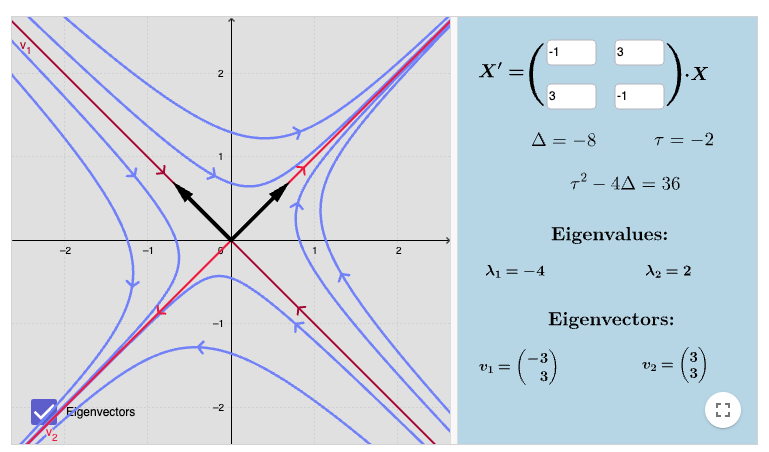
\includegraphics[width=5in]{Images/ImgPhasePlane1331.png}
        \end{center}         
    } 
    \else 
        \begin{center}
        \begin{tikzpicture}[scale=0.65]
        \draw[very thick, ->] (-3, 0) -- (3.25, 0);
        \draw[very thick, ->] (0, -3) -- (0, 3.25);
        \end{tikzpicture}
        \end{center}    
    \fi    

    \part Classify the critical point according to stability and type. 
    
    \ifnum \Solutions=1 {\color{DarkBlue} 
    \textbf{Solutions:} unstable saddle
    } 
    \else 
    \vspace{3cm}
    \fi
    
\end{parts}
\fi







\ifnum \Version=7
    \question[4] Consider the IVP $$\vec x \, ' = A\vec x, \quad A = \begin{pmatrix} -3&2\\2&-3 \end{pmatrix}, \quad \vec x = \begin{pmatrix} x(t)\\y(t)\end{pmatrix}, \quad \vec x(0) = \begin{pmatrix} 2\\-2 \end{pmatrix}$$ The eigenvalues of $A$ are $\lambda_1 = -1$ and $\lambda_2 = -5$. 
    \begin{parts}
        \part Determine the eigenvectors of $A$. Please show your work. 
        
        \ifnum \Solutions=1 {\color{DarkBlue} 
        \textbf{Solutions:}
        For $\lambda_1$, with $\ast =$ not needed, we obtain
        \begin{align}
            A - \lambda_1 I = \begin{pmatrix} -3& 3\\\ast &\ast\end{pmatrix} \ \Rightarrow \ v_1 = \begin{pmatrix} 1\\1 \end{pmatrix}
        \end{align}
        For $\lambda_2$:
        \begin{align}
            A - \lambda_2 I = \begin{pmatrix} 3&3\\\ast& \ast \end{pmatrix} \ \Rightarrow \ v_2 = \begin{pmatrix} -1\\1 \end{pmatrix}
        \end{align}    
        } 
        \else 
            \vspace{6cm}   
        \fi        
        \part Use the given eigenvalues and the eigenvectors that you calculated in part (a) to solve the IVP.  
        
        \ifnum \Solutions=1 {\color{DarkBlue} 
        \textbf{Solutions:} the general solution to the DE is:
        $$\vec x = c_1 e^{-t}\begin{pmatrix} 1\\1\end{pmatrix} + c_2e^{-5t} \begin{pmatrix} -1\\1\end{pmatrix}$$
        Use initial condition:
        \begin{align}
            \begin{pmatrix} 2\\-2\end{pmatrix} &= c_1\begin{pmatrix}1\\1 \end{pmatrix}+ c_2 \begin{pmatrix} -1\\1\end{pmatrix} \ \Rightarrow \ c_1 = 0, c_2 = -2 \ \Rightarrow \ 
            \vec x (t) = -2e^{-5t} \begin{pmatrix} -1\\1\end{pmatrix}
        \end{align}
        } 
        \else 
        \vspace{7cm}
    \fi
    \part Sketch the phase portrait of the system on the axes below. Please indicate the direction of motion on your solution curves and draw the eigenspaces corresponding to real eigenvalues (if any). Please also label your axes. 
    
    \ifnum \Solutions=1 {\color{DarkBlue}   
    \textbf{Solutions:}
        \begin{center}
        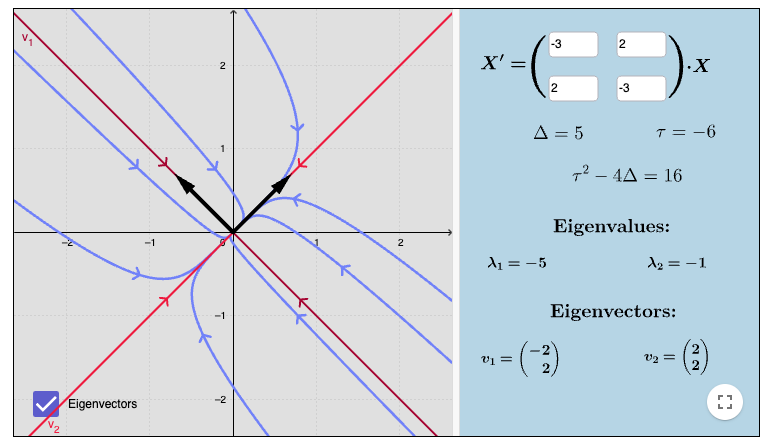
\includegraphics[width=5in]{Images/ImgPhasePlane3223.png}
        \end{center}         
    } 
    \else 
        \begin{center}
        \begin{tikzpicture}[scale=0.65]
        \draw[very thick, ->] (-3, 0) -- (3.25, 0);
        \draw[very thick, ->] (0, -3) -- (0, 3.25);
        \end{tikzpicture}
        \end{center}    
    \fi    

    \part Classify the critical point according to stability and type. 
    
    \ifnum \Solutions=1 {\color{DarkBlue} 
    \textbf{Solutions:} stable node
    } 
    \else 
    \vspace{3cm}
    \fi

\end{parts}
\fi
        \ifnum \Version=1
\question[10] Consider the first order, constant coefficient, linear initial value problem $\vec x \, ' = A\vec x, \ \vec x (0) = \vec x_0$, where $\vec x \, ' = A\vec x$ and $\vec x = \vec x(t)$. The vector $\vec x_0$, and the eigenvalues and eigenvectors of $A$ are as follows. 
$$\lambda_1 = -3, \ \vec v_1 = \begin{pmatrix}1\\0\\0 \end{pmatrix} , \quad \lambda_2 = -4, \ \vec v_2 = \begin{pmatrix} 0\\1\\2 \end{pmatrix}, \quad \lambda_3 = -4, \ \vec v_3 = \begin{pmatrix} 0\\0\\1\end{pmatrix}, \quad \vec x_0 = \begin{pmatrix} 2\\4\\6\end{pmatrix}$$
\begin{parts}
    \part Write down the general solution to the system of differential equations in terms of real-valued functions. 
    \vspace{4cm}
    \part Solve the initial value problem. Please state the solution to the initial value problem clearly and please show your work. 
\end{parts}
\fi






\ifnum \Version=6
\newpage
\question[4] Consider the first order, constant coefficient, linear IVP $\vec x \, ' = A\vec x, \ \vec x (0) = \vec x_0$, where $\vec x \, ' = A\vec x$ and $\vec x = \vec x(t)$. The eigenvalues and eigenvectors of $A$, and $\vec x_0$, are below. 
$$\lambda_1 = -4, \  v_1 = \begin{pmatrix}1\\0\\0 \end{pmatrix} , \quad \lambda_2 = -2+3i, \  v_2 = \begin{pmatrix} 0\\2\\i \end{pmatrix}, \quad \lambda_3 = \bar{\lambda_2}, \ v_3 = \bar{v_2}, \quad \vec x_0 = \begin{pmatrix} 9\\2\\0\end{pmatrix}$$
\begin{parts}
    \part Write down the general solution to the system of differential equations $\vec x \, ' = A \vec x$ in terms of real-valued functions. 
    \ifnum \Solutions=0 \vspace{8cm} \fi
    \part Solve the initial value problem. Please state the solution to the initial value problem clearly and please show your work. 
    \ifnum \Solutions=0 \vfill \fi
\end{parts}
\ifnum \Solutions=1 {\color{DarkBlue} 
\textbf{Solutions:} the general solution is
\begin{align*}
    \vec x = c_1 e^{-4t}\begin{pmatrix} 1\\0\\0\end{pmatrix} 
    + c_2e^{-2t}\left(\begin{pmatrix} 0\\2\\0\end{pmatrix} \cos(3t) - \begin{pmatrix} 0\\0\\1  \end{pmatrix} \sin(3t) \right) 
    + c_3e^{-2t}\left(\begin{pmatrix} 0\\2\\0\end{pmatrix} \sin(3t) + \begin{pmatrix} 0\\0\\1  \end{pmatrix} \cos(3t) \right) 
\end{align*}
When $t=0$ this reduces to
\begin{align*}
    \vec x(0) = \begin{pmatrix} 9\\2\\0\end{pmatrix} = c_1 \begin{pmatrix} 1\\0\\0\end{pmatrix} 
    + c_2 \begin{pmatrix} 0\\2\\0\end{pmatrix} 
    + c_3  \begin{pmatrix} 0\\0\\1  \end{pmatrix}  
\end{align*}
Thus $c_1= 9$, $c_2=1$, $c_3= 0$.
\begin{align*}
    \vec x = 9 e^{-4t}\begin{pmatrix} 1\\0\\0\end{pmatrix} 
    + e^{-2t}\left(\begin{pmatrix} 0\\2\\0\end{pmatrix} \cos(3t) - \begin{pmatrix} 0\\0\\1  \end{pmatrix} \sin(3t) \right) \end{align*}
} 
\else 
\newpage
\fi
\fi


\ifnum \Version=7
\newpage
\question[4] Consider the first order, constant coefficient, linear IVP $\vec x \, ' = A\vec x, \ \vec x (0) = \vec x_0$, where $\vec x \, ' = A\vec x$ and $\vec x = \vec x(t)$. The eigenvalues and eigenvectors of $A$, and $\vec x_0$, are below. 
$$\lambda_1 = -4, \  v_1 = \begin{pmatrix}1\\0\\0 \end{pmatrix} , \quad \lambda_2 = -2+3i, \  v_2 = \begin{pmatrix} 0\\2\\9i \end{pmatrix}, \quad \lambda_3 = \bar{\lambda_2}, \ v_3 = \bar{v_2}, \quad \vec x_0 = \begin{pmatrix} 5\\0\\36\end{pmatrix}$$
\begin{parts}
    \part Write down the general solution to the system of differential equations $\vec x \, ' = A \vec x$ in terms of real-valued functions. 
    \ifnum \Solutions=0 \vspace{8cm} \fi
    \part Solve the initial value problem. Please state the solution to the initial value problem clearly and please show your work. 
    \ifnum \Solutions=0 \vfill \fi
\end{parts}
\ifnum \Solutions=1 {\color{DarkBlue} 
\textbf{Solutions:} the general solution is
\begin{align*}
    \vec x = c_1 e^{-4t}\begin{pmatrix} 1\\0\\0\end{pmatrix} 
    + c_2e^{-2t}\left(\begin{pmatrix} 0\\2\\0\end{pmatrix} \cos(3t) - \begin{pmatrix} 0\\0\\9  \end{pmatrix} \sin(3t) \right) 
    + c_3e^{-2t}\left(\begin{pmatrix} 0\\2\\0\end{pmatrix} \sin(3t) + \begin{pmatrix} 0\\0\\9  \end{pmatrix} \cos(3t) \right) 
\end{align*}
When $t=0$ this reduces to
\begin{align*}
    \vec x(0) = \begin{pmatrix} 5\\0\\36\end{pmatrix} = c_1 \begin{pmatrix} 1\\0\\0\end{pmatrix} 
    + c_2 \begin{pmatrix} 0\\2\\0\end{pmatrix} 
    + c_3  \begin{pmatrix} 0\\0\\9  \end{pmatrix}  
\end{align*}
Thus $c_1= 5$, $c_2=0$, $c_3= 4$.
\begin{align*}
    \vec x = 5 e^{-4t}\begin{pmatrix} 1\\0\\0\end{pmatrix} 
        + 4e^{-2t}\left(\begin{pmatrix} 0\\2\\0\end{pmatrix} \sin(3t) + \begin{pmatrix} 0\\0\\9  \end{pmatrix} \cos(3t) \right) 
\end{align*}
} 
\else 
\newpage
\fi
\fi




        \ifnum \Version=1
\newpage 
\question[5] Consider the differential equation

    $$y'' + p(t)y' + q(t)y = 16t^3, \quad y=y(t)$$    
    
    Solutions to the corresponding homogeneous problem are $y_1 = t$ and $y_2 = t^3$. 

    \begin{parts}
        \part Determine a particular solution to the differential equation using variation of parameters. Do not use the method of undetermined coefficients. 
        \ifnum \Solutions=0 
        \vspace{16cm}
        \fi
        \part State the general solution to the differential equation.
    \end{parts}
    \ifnum \Solutions=1 {\color{DarkBlue} 
    \begin{enumerate}
        \item[a)] The Wronskian is
    \begin{align}
        W = \det \begin{pmatrix} t&t^3\\1&3t^2\end{pmatrix} = 2t^3
    \end{align}
    To apply the formulas for the variation of parameters method for a second order DE we also use
    \begin{align}
        y_1 & = t \\
        y_2 &= t^3 \\
        g &= 16t^3 
    \end{align}
    Applying the formulas for $v_1$ and $v_2$ we obtain
    \begin{align}
        v_1 &= - \int \frac{y_2(t)g(t)}{W[y_1,y_2]}dt = - \int \frac{t^3 \cdot 16t^3}{2t^3} dt = - \int 8 t^3 \, dt = -2t^4 + k_1\\
        v_2 &= \int \frac{y_1(t)g(t)}{W[y_1,y_2]} dt = \int \frac{t\cdot16t^3}{2t^3} dt = \int 8 t \, dt = 4t^2 + k_2
    \end{align}
    The arbitrary constants of integration, $k_1$ and $k_2$, in the above are actually not necessary. In the end they will only produce redundant terms because they are solutions to the homogeneous equation. But it is OK to leave them in the expressions for $v_1$ and $v_2$, in the expression for $y_p$, and the expression for $y$. The expression for $y_p$ becomes
    \begin{align}
        y_p &= v_1y_1 + v_2y_2 
        = (-2t^4 )\cdot t + (4t^2 ) t^3 
        = 2t^5
    \end{align}
    \item [b)] The general solution to the differential equation is
    \begin{align}
        y &= y_h + y_p \\
        &= c_1y_1 + c_2y_2 + v_1y_1 + v_2y_2 \\
        &= c_1t +c_2t^3 + 2t^5 
    \end{align}
    \end{enumerate}
    } 
    \else 
    \fi    
\fi



\ifnum \Version=2
\ifnum \Solutions=0 \newpage \fi
\question[5] Consider the first order constant-coefficient system below. 
    
\[\vec{x}\, ' = P\vec {x} + \vec g, \quad \vec g = \begin{pmatrix} 9\\2\end{pmatrix}\] 

Matrix $P$ is $2\times2$ with real entries. A fundamental set of solutions to the corresponding homogeneous problem is given by the following vectors.   
\[\vec{x}_{1}(t)=e^{t}\begin{pmatrix}1\\0\end{pmatrix},\qquad \vec{x}_{2}(t)=e^{2t}\begin{pmatrix}4\\1\end{pmatrix}\]  

    \begin{parts}
        \part Determine a particular solution to the differential equation using variation of parameters. Do not use the method of undetermined coefficients. 
        \ifnum \Solutions=0 
        \vspace{16cm}
        \fi
        \part State the general solution to the system of differential equations.
    \end{parts}
    
    \ifnum \Solutions=1 {\color{DarkBlue} \textit{Solution.} 
    We will use the formula given in the formula page
$$\vec x_p(t) = \mathbf{X}(t) \int \mathbf{X} ^ {-1} (t) \vec{g} (t) dt.$$
The fundamental matrix and its inverse are:
\begin{align}
    \mathbf{X} (t) 
    &= \begin{pmatrix} \vec{x}_{1} & \vec{x}_{2}\end{pmatrix} 
    = \begin{pmatrix} e ^ {t} & 4e ^ {2t}\\ 0 &   e ^ {2t} \end{pmatrix} \\
    \mathbf{X}^{-1} 
    &= \frac{1}{e^{3t}}\begin{pmatrix} e^{2t} & -4e^{2t} \\0 & e^{t}\end{pmatrix} 
    = \begin{pmatrix} e^{-t} & -4e^{-t} \\0 & e^{-2t} \end{pmatrix}
\end{align}
The inverse was obtained using the formula for the inverse of a $2\times 2$ matrix. 
\begin{align}
    \mathbf{X} ^ {-1} (t) \vec{g}(t) 
    &= \begin{pmatrix} e^{-t} & -4e^{-t} \\0 & e^{-2t} \end{pmatrix} \begin{pmatrix} 9\\2 \end{pmatrix} 
    = \begin{pmatrix} e^{-t} \\ 2e^{-2t}\end{pmatrix} \\
    \int \mathbf{X} ^ {-1} (t) \vec{g}(t) dt 
    &= \int \begin{pmatrix} e^{-t} \\ 2e^{2t}\end{pmatrix} dt = \begin{pmatrix} -e^{-t} \\ -e^{-2t} \end{pmatrix} \\
    \vec x_p = \mathbf{X}(t) \int \mathbf{X} ^ {-1} (t) \vec{g}(t) dt 
    &= \begin{pmatrix} e^{t} & 4e^{2t}\\ 0 & e^{2t} \end{pmatrix}\begin{pmatrix} -e^{-t} \\ -e^{-2t} \end{pmatrix}
    = \begin{pmatrix} -5 \\ -1 \end{pmatrix}
\end{align}
The particular solution is a constant vector. 
\begin{align}
    \vec x_p =  \begin{pmatrix} -5 \\ -1 \end{pmatrix} = - \begin{pmatrix} 5 \\ 1 \end{pmatrix}
\end{align}

The general solution is the homogeneous solution plus the particular solution. 
\begin{align}
    \vec x = \vec x_h + \vec x_p = c_1e^{t}\begin{pmatrix}1\\0\end{pmatrix} + c_2e^{2t}\begin{pmatrix}4\\1\end{pmatrix} - \begin{pmatrix} 5\\1\end{pmatrix}
\end{align}

    } 
   \else
   \fi

\fi 





\ifnum \Version=3
\ifnum \Solutions=0 \newpage \fi
\question[5] Consider the first order constant-coefficient system below. 
    
\[\vec{x}\, ' = P\vec {x} + \vec g, \quad \vec g = \begin{pmatrix} 5\\2\end{pmatrix}\] 

Matrix $P$ is $2\times2$ with real entries. A fundamental set of solutions to the corresponding homogeneous problem is given by the following vectors.   
\[\vec{x}_{1}(t)=e^{-t}\begin{pmatrix}1\\0\end{pmatrix},\qquad \vec{x}_{2}(t)=e^{-2t}\begin{pmatrix}2\\1\end{pmatrix}\]  

    \begin{parts}
        \part Determine a particular solution to the differential equation using variation of parameters. Do not use the method of undetermined coefficients. 
        \ifnum \Solutions=0 
        \vspace{16cm}
        \fi
        \part State the general solution to the system of differential equations.
    \end{parts}
    
    \ifnum \Solutions=1 {\color{DarkBlue} \textit{Solution.} 
    We will use the formula
$$\vec x_p(t) = \mathbf{X}(t) \int \mathbf{X} ^ {-1} (t) \vec{g} (t) dt.$$
The fundamental matrix and its inverse are:
\begin{align}
    \mathbf{X} (t) &= \begin{pmatrix} \vec{x}_{1} & \vec{x}_{2}\end{pmatrix} = \begin{pmatrix} 
    e ^ {-t} & 2e ^ {-2t}\\ 0 &   e ^ {-2t} \end{pmatrix} \\
    \mathbf{X}^{-1} &= \frac{1}{e^{-3t}}\begin{pmatrix} e^{-2t} & -2e^{-2t} \\0 & e^{-t}\end{pmatrix} = \begin{pmatrix} e^t & -2e^t \\0 & e^{2t} \end{pmatrix}
\end{align}
The inverse was obtained using the formula for the inverse of a $2\times 2$ matrix we obtain. Then:
\begin{align}
    \mathbf{X} ^ {-1} (t) \vec{g}(t) &= \begin{pmatrix} e^t & -2e^t \\0 & e^{2t} \end{pmatrix} \begin{pmatrix} 5\\2 \end{pmatrix} = \begin{pmatrix} e^t \\ 2e^{2t}\end{pmatrix} \\
    \int \mathbf{X} ^ {-1} (t) \vec{g}(t) dt &= \int \begin{pmatrix} e^t \\ 2e^{2t}\end{pmatrix} dt = \begin{pmatrix} e^t \\ e^{2t} \end{pmatrix} \\
    \vec x_p = \mathbf{X}(t) \int \mathbf{X} ^ {-1} (t) \vec{g}(t) dt &= \begin{pmatrix} 
    e ^ {-t} & 2e ^ {-2t}\\ 0 &   e ^ {-2t} \end{pmatrix} \begin{pmatrix} e^t \\ e^{2t} \end{pmatrix} = \begin{pmatrix} 3 \\ 1 \end{pmatrix}
\end{align}
The particular solution is a constant vector. 
\begin{align}
    \vec x_p =  \begin{pmatrix} 3 \\ 1 \end{pmatrix}
\end{align}

The general solution is the homogeneous solution plus the particular solution. 
\begin{align}
    \vec x = \vec x_h + \vec x_p = c_1e^{-t}\begin{pmatrix}1\\0\end{pmatrix} + c_2e^{-2t}\begin{pmatrix}2\\1\end{pmatrix} + \begin{pmatrix} 3\\1\end{pmatrix}
\end{align}

    } 
   \else
   \fi

\fi 





\ifnum \Version=4
\ifnum \Solutions=0 \newpage \fi
\question[5] Consider the first order constant-coefficient system below. 
\[\vec{x}\, ' = P\vec {x} + \vec g, \quad \vec g = \begin{pmatrix} 14\\3\end{pmatrix}\] 

Matrix $P$ is $2\times2$ with real entries. A fundamental set of solutions to the corresponding homogeneous problem is given by the following vectors.   
\[\vec{x}_{1}(t)=e^{-2t}\begin{pmatrix}1\\0\end{pmatrix},\qquad \vec{x}_{2}(t)=e^{-3t}\begin{pmatrix}4\\1\end{pmatrix}\]  

    \begin{parts}
        \part Determine a particular solution to the differential equation using variation of parameters. Do not use the method of undetermined coefficients. 
        \ifnum \Solutions=0 
        \vspace{16cm}
        \fi
        \part State the general solution to the system of differential equations.
    \end{parts}
    
    \ifnum \Solutions=1 {\color{DarkBlue} \textit{Solution.} 
    We will use the formula
$$\vec x_p(t) = \mathbf{X}(t) \int \mathbf{X} ^ {-1} (t) \vec{g} (t) dt.$$
The fundamental matrix and its inverse are:
\begin{align}
    \mathbf{X} (t) &= \begin{pmatrix} \vec{x}_{1} & \vec{x}_{2}\end{pmatrix} 
    = \begin{pmatrix}  e ^ {-2t} & 4e ^ {-3t}\\ 0 &   e ^ {-3t} \end{pmatrix} \\
    \mathbf{X}^{-1} 
    &= \frac{1}{e^{-5t}}\begin{pmatrix} e^{-3t} & -4e^{-3t} \\0 & e^{-2t}\end{pmatrix} = e^{5t}\begin{pmatrix} e^{-3t} & -4e^{-3t} \\0 & e^{-2t}\end{pmatrix} 
    = \begin{pmatrix} e^{2t} & -4e^{2t} \\0 & e^{3t} \end{pmatrix}
\end{align}
The inverse was obtained using the formula for the inverse of a $2\times 2$ matrix we obtain. Then:
\begin{align}
    \vec x_p = \mathbf{X}(t) \int \mathbf{X} ^ {-1} (t) \vec{g}(t) \, dt 
    &= \mathbf{X}(t) \int \begin{pmatrix} e^{2t} & -4e^{2t} \\0 & e^{3t} \end{pmatrix} \begin{pmatrix} 14 \\ 3 \end{pmatrix} \, dt \\
    & = \mathbf{X}(t) \int \begin{pmatrix} 2e^{2t} \\ 3e^{3t}\end{pmatrix} \, dt \\
    & = \mathbf{X}(t)  \begin{pmatrix} e^{2t} \\ e^{3t}\end{pmatrix} \\
    & = \begin{pmatrix}  e ^ {-2t} & 4e ^ {-3t}\\ 0 &   e ^ {-3t} \end{pmatrix}  \begin{pmatrix} e^{2t} \\ e^{3t}\end{pmatrix} \\
    & =  \begin{pmatrix} 1 + 4 \\ 0 + 1\end{pmatrix} 
\end{align}
The particular solution is a constant vector $\displaystyle \vec x_p =  \begin{pmatrix} 5 \\ 1 \end{pmatrix}$. The general solution is the homogeneous solution plus the particular solution. 
\begin{align}
    \vec x = \vec x_h + \vec x_p = c_1e^{-2t}\begin{pmatrix}1\\0\end{pmatrix} + c_2e^{-3t}\begin{pmatrix}4\\1\end{pmatrix} + \begin{pmatrix} 5\\1\end{pmatrix}
\end{align}

    } 
   \else
   \fi

\fi 








\ifnum \Version=5
\question[5] Determine the general solution to the differential equation. 
$$y'' + 4y = 100te^{-t}, \quad y=y(t)$$
\ifnum \Solutions=1 {\color{DarkBlue} \\[12pt] 
The homogeneous equation has the characteristic equation
$$\lambda ^2+4\lambda = 0$$
The roots are $\lambda= 0$, $\lambda = -4$, so the homogeneous solution is
$$y_h = c_1 e^{0t} + c_2 e^{-4t} = c_1 + c_2 e^{-4t}$$
We can use undetermined coefficients to identify the particular solution. With undetermined coefficients we can try a solution of the form $y_p = (At+B)e^{-t}$. To substitute this expression for the particular solution to the given differential equation, we differentiate twice to obtain:
\begin{align}
    y_p ' &= Ae^{-t} - Ate^{-t} - Be^{-t} \\
    y_p'' &= -2Ae^{-t} +Ate^{-t} + Be^{-t}
\end{align}
Substituting these expressions into the differential equation we have:
\begin{align}
    0 &= y'' + 4y \\
    0 &= (-2Ae^{-t} +Ate^{-t} +    Be^{-t}) +4 (Ae^{-t} - Ate^{-t} - Be^{-t}) \\ 
    0 &= 2Ae^{-t} - 4Ate^{-t} + Be^{-t}
\end{align}
By comparison, we obtain
$$ A = , B = 0$$
The full solution to the DE is NEED TO FINISH SOLUTIONS
$$y = y_h + y_p = c_1y_1  + c_2y_2 + y_p = c_1 + c_2 e^{-4t} + $$
} 
\else 
\vspace{3cm}
\fi
\fi 




\ifnum \Version=6
\newpage 
\question[4] Consider the differential equation

    $$y'' + p(t)y' + q(t)y = 12e^{-t}, \quad y=y(t)$$    
    
    Solutions to the corresponding homogeneous problem are $y_1 = e^{-t}, \ y_2 = te^{-t}$. 

    \begin{parts}
        \part Determine a particular solution to the differential equation using variation of parameters. Do not use the method of undetermined coefficients. 
        \ifnum \Solutions=0 
        \vspace{16cm}
        \fi
        \part State the general solution to the differential equation.
    \end{parts}
    \ifnum \Solutions=1 {\color{DarkBlue} 
    \begin{enumerate}
        \item[a)] The Wronskian is
    \begin{align}
        W = \det \begin{pmatrix} e^{-t}&te^{-t}\\-e^{-t}&e^{-t}-te^{-t}\end{pmatrix} = e^{-t}(e^{-t}-te^{-t})+te^{-2t} = e^{-2t}(1 -t+t) = e^{-2t}
    \end{align}
    To apply the formulas for the variation of parameters method for a second order DE we also use
    \begin{align}
        y_1 & = e^{-t} \\
        y_2 &= te^{-t} \\
        g &= 12e^{-t}
    \end{align}
    Applying the formulas for $v_1$ and $v_2$ we obtain
    \begin{align}
        v_1 &= - \int \frac{y_2(t)g(t)}{W[y_1,y_2]}dt = - \int \frac{te^{-t} \cdot 12e^{-t}}{e^{-2t}} dt = - \int 12t \, dt = -6t^2 + k_1\\
        v_2 &= \int \frac{y_1(t)g(t)}{W[y_1,y_2]} dt = \int \frac{e^{-t}\cdot12e^{-t}}{e^{-2t}} dt = \int 12 \, dt = 12t + k_2
    \end{align}
    The arbitrary constants of integration, $k_1$ and $k_2$, in the above are actually not necessary. In the end they will only produce redundant terms because they are solutions to the homogeneous equation. But it is OK to leave them in the expressions for $v_1$ and $v_2$, in the expression for $y_p$, and the expression for $y$. The expression for $y_p$ becomes
    \begin{align}
        y_p &= v_1y_1 + v_2y_2 
        = -6t^2 e^{-t} + 12t^2e^{-t} = 6t^2e^{-t}
    \end{align}
    \item [b)] The general solution to the differential equation is
    \begin{align}
        y &= y_h + y_p \\
        &= c_1y_1 + c_2y_2 + v_1y_1 + v_2y_2 \\
        &= c_1e^{-t} +c_2te^{-t} + 6t^2e^{-t}
    \end{align}
    \end{enumerate}
    } 
    \else 
    \fi    
\fi






\ifnum \Version=7
\newpage 
\question[4] Consider the differential equation

    $$y'' + p(t)y' + q(t)y = 12e^{-t}, \quad y=y(t)$$    
    
    Solutions to the corresponding homogeneous problem are $y_1 = e^{-t}, \ y_2 = te^{-t}$. 

    \begin{parts}
        \part Determine a particular solution to the differential equation using variation of parameters. Do not use the method of undetermined coefficients. 
        \ifnum \Solutions=0 
        \vspace{16cm}
        \fi
        \part State the general solution to the differential equation.
    \end{parts}
    \ifnum \Solutions=1 {\color{DarkBlue} 
    \begin{enumerate}
        \item[a)] The Wronskian is
    \begin{align}
        W = \det \begin{pmatrix} e^{-t}&te^{-t}\\-e^{-t}&e^{-t}-te^{-t}\end{pmatrix} = e^{-t}(e^{-t}-te^{-t})+te^{-2t} = e^{-2t}(1 -t+t) = e^{-2t}
    \end{align}
    To apply the formulas for the variation of parameters method for a second order DE we also use
    \begin{align}
        y_1 & = e^{-t} \\
        y_2 &= te^{-t} \\
        g &= 12e^{-t}
    \end{align}
    Applying the formulas for $v_1$ and $v_2$ we obtain
    \begin{align}
        v_1 &= - \int \frac{y_2(t)g(t)}{W[y_1,y_2]}dt = - \int \frac{te^{-t} \cdot 12e^{-t}}{e^{-2t}} dt = - \int 12t \, dt = -6t^2 + k_1\\
        v_2 &= \int \frac{y_1(t)g(t)}{W[y_1,y_2]} dt = \int \frac{e^{-t}\cdot12e^{-t}}{e^{-2t}} dt = \int 12 \, dt = 12t + k_2
    \end{align}
    The arbitrary constants of integration, $k_1$ and $k_2$, in the above are actually not necessary. In the end they will only produce redundant terms because they are solutions to the homogeneous equation. But it is OK to leave them in the expressions for $v_1$ and $v_2$, in the expression for $y_p$, and the expression for $y$. The expression for $y_p$ becomes
    \begin{align}
        y_p &= v_1y_1 + v_2y_2 
        = -6t^2 e^{-t} + 12t^2e^{-t} = 6t^2e^{-t}
    \end{align}
    \item [b)] The general solution to the differential equation is
    \begin{align}
        y &= y_h + y_p \\
        &= c_1y_1 + c_2y_2 + v_1y_1 + v_2y_2 \\
        &= c_1e^{-t} +c_2te^{-t} + 6t^2e^{-t}
    \end{align}
    \end{enumerate}
    } 
    \else 
    \fi    
\fi



        \ifnum \Version=1
\question[1] You do not need to show your work for this question. Consider the nonlinear system below.
\begin{align*}
    \dxdt &= (x-1)(y-5) , \qquad \dydt = y-x^2-1
\end{align*}
How many critical points does the system have? \framebox{\strut\hspace{1cm}}
\ifnum \Solutions=1 {\color{DarkBlue} \\[12pt] 
For a point to critical point, we need $x' = y' = 0$. If $x'$ is zero, then either $x=1$ or $y=5$. Likewise if $y'=0$ then $y=x^2+1$. The curves are shown below. The green lines are the x nullclines, and the red curve is the y nullcline. There are exactly three critical points. 
    \begin{center}
    \begin{tikzpicture}[scale=0.75]
    \draw[thick, ->] (-6, 0) -- (6.25, 0);
    \draw[thick, ->] (0, -1) -- (0, 6.25);
    \node[overlay, below] at (6, -0.2) {$x$};
    \node[overlay, below] at (-0.6, 6) {$y$};   
    \draw[very thick,DarkGreen, -] (1, 6) -- (1, -1);        
    \draw[very thick,DarkGreen, -] (-6, 5) -- (6, 5);   
    \draw[DarkRed, line width = 0.50mm]   plot[smooth,domain=-2.1:2.1] (\x, {\x*\x+1});
    \filldraw[black] (2,5) circle (4pt) node[anchor=south west]{(2,5)};
    \filldraw[black] (-2,5) circle (4pt) node[anchor=south west]{(-2,5)};
    \filldraw[black] (1,2) circle (4pt) node[anchor=south west]{(1,2)};
    \end{tikzpicture}
    \end{center}         
} 
\else 
\vspace{3cm}
\fi    
\fi 


\ifnum \Version=2
\question[1] You do not need to show your work for this question. Consider the nonlinear system below.
\begin{align*}
    \dxdt &= (y-1)(y-5)(x-1) , \qquad \dydt = y-x^2-1
\end{align*}
How many critical points does the system have? \framebox{\strut\hspace{1cm}}
\ifnum \Solutions=1 {\color{DarkBlue} \\[12pt] 
For a point to critical point, we need $x' = y' = 0$. If $x'$ is zero, then either $x=1$, $y=1$ or $y=5$. Likewise if $y'=0$ then $y=x^2+1$. The curves are shown below. The green lines are the x nullclines, and the red curve is the y nullcline. There are exactly four critical points. 
    \begin{center}
    \begin{tikzpicture}[scale=0.75]
    \draw[thick, ->] (-6, 0) -- (6.25, 0);
    \draw[thick, ->] (0, -1) -- (0, 6.25);
    \node[overlay, below] at (6, -0.2) {$x$};
    \node[overlay, below] at (-0.6, 6) {$y$};   
    \draw[very thick,DarkGreen, -] (-6, 1) -- (6, 1);   
    \draw[very thick,DarkGreen, -] (-6, 5) -- (6, 5);   
    \draw[very thick,DarkGreen, -] (1, -1) -- (1, 6);   
    \draw[DarkRed, line width = 0.50mm]   plot[smooth,domain=-2.1:2.1] (\x, {\x*\x+1});
    \filldraw[black] (2,5) circle (4pt) node[anchor=south west]{(2,5)};
    \filldraw[black] (1,2) circle (4pt) node[anchor=south west]{(1,2)};
    \filldraw[black] (-2,5) circle (4pt) node[anchor=south west]{(-2,5)};
    \filldraw[black] (0,1) circle (4pt) node[anchor=south west]{(0,1)};
    \end{tikzpicture}
    \end{center}         
} 
\else 
\vspace{3cm}
\fi    
\fi 



\ifnum \Version=3
\question[1] You do not need to show your work for this question. Consider the nonlinear system below.
\begin{align*}
    \dxdt &= (x-1)(y-5) , \qquad \dydt = y-x^2-1
\end{align*}
How many critical points does the system have? \framebox{\strut\hspace{1cm}}
\ifnum \Solutions=1 {\color{DarkBlue} \\[12pt] 
For a point to critical point, we need $x' = y' = 0$. If $x'$ is zero, then either $x=1$ or $y=5$. Likewise if $y'=0$ then $y=x^2+1$. The curves are shown below. The green lines are the x nullclines, and the red curve is the y nullcline. There are exactly three critical points. 
    \begin{center}
    \begin{tikzpicture}[scale=0.75]
    \draw[thick, ->] (-6, 0) -- (6.25, 0);
    \draw[thick, ->] (0, -1) -- (0, 6.25);
    \node[overlay, below] at (6, -0.2) {$x$};
    \node[overlay, below] at (-0.6, 6) {$y$};   
    \draw[very thick,DarkGreen, -] (1, 6) -- (1, -1);        
    \draw[very thick,DarkGreen, -] (-6, 5) -- (6, 5);   
    \draw[DarkRed, line width = 0.50mm]   plot[smooth,domain=-2.1:2.1] (\x, {\x*\x+1});
    \filldraw[black] (2,5) circle (4pt) node[anchor=south west]{(2,5)};
    \filldraw[black] (-2,5) circle (4pt) node[anchor=south west]{(-2,5)};
    \filldraw[black] (1,2) circle (4pt) node[anchor=south west]{(1,2)};
    \end{tikzpicture}
    \end{center}         
} 
\else 
\vspace{1cm}
\fi    
\fi 


\ifnum \Version=4
\question[1] You do not need to show your work for this question. Consider the nonlinear system below.
\begin{align*}
    \dxdt &= (y-4)(x-1) , \qquad \dydt = y-x^2
\end{align*}
Where are the critical points of this system located? % \framebox{\strut\hspace{5cm}}
\ifnum \Solutions=1 {\color{DarkBlue} \\[12pt] 
For a point to critical point, we need $x' = y' = 0$. If $x'$ is zero, then either $x=1$, or $y=4$. Likewise if $y'=0$ then $y=x^2$. The curves are shown below. The green lines are the x nullclines, and the red curve is the y nullcline. There are exactly three critical points. We care not for the points where green crosses green. 
    \begin{center}
    \begin{tikzpicture}[scale=0.75]
    \draw[thick, ->] (-6, 0) -- (6.25, 0);
    \draw[thick, ->] (0, -1) -- (0, 6.25);
    \node[overlay, below] at (6, -0.2) {$x$};
    \node[overlay, below] at (-0.6, 6) {$y$};   
    \draw[very thick,DarkGreen, -] (1, -1) -- (1, 4.5);   
    \draw[very thick,DarkGreen, -] (-4, 4) -- (4, 4);   
    \draw[DarkRed, line width = 0.50mm]   plot[smooth,domain=-2.1:2.1] (\x, {\x*\x});
    \filldraw[black] (1,1) circle (4pt) node[anchor=south west]{(1,1)};
    \filldraw[black] (2,4) circle (4pt) node[anchor=south west]{(2,4)};
    \filldraw[black] (-2,4) circle (4pt) node[anchor=south west]{(-2,4)};
    \end{tikzpicture}
    \end{center}         
} 
\else 
\vspace{3cm}
\fi    
\fi 



\ifnum \Version=6
\newpage
\question[3] You do not need to show your work for this question. Consider the nonlinear system below.
\begin{align*}
    \dxdt &= x(4-2x-y) , \qquad \dydt = y(2-2x-y)
\end{align*}
You can assume that $x$ and $y$ represent populations, so $x\ge0$ and $y\ge0$. 
\begin{parts}
    \part Write down the equations of the lines that correspond to where solution curves are horizontal. 
    
    \ifnum \Solutions=1 {\color{DarkBlue} 
    \textbf{Solutions:} horizontal where $y'=0$, which occurs on the lines $y=0$ and $y=2-2x$. 
    } 
    \else 
    \vspace{2cm}
    \fi
    \part Where are the critical points of this system located? 

    \ifnum \Solutions=1 {\color{DarkBlue} 
    \textbf{Solutions:} by inspection the only CPs are at $(0,0)$, $(0,2)$, $(2,0)$. 
    } 
    \else 
    \vspace{4cm}
    \fi
    \part Sketch the nullclines of the system on the axes below. Clearly indicate the critical points. 
    \ifnum \Solutions=1 {\color{DarkBlue} \\[12pt] 
        Green lines are the $x-$nullclines, red lines are the $y-$nullclines.
        \begin{center}
        \begin{tikzpicture}[scale=1]
        \draw[thick, ->] (-1, 0) -- (6.25, 0);
        \draw[thick, ->] (0, -1) -- (0, 6.25);
        \node[overlay, below] at (5, -0.2) {$x$};
        \node[overlay, below] at (-0.6, 6) {$y$};   
        \draw[ultra thick,DarkRed, -] (0, 0) -- (5, 0);        
        \draw[ultra thick,DarkGreen, -] (0,4) -- (2, 0);   
        \draw[ultra thick,DarkRed, -] (0, 2) -- (1, 0);        
        \draw[ultra thick,DarkGreen, -] (0, 0) -- (0, 5);      
        \filldraw[black] (0,0) circle (4pt) node[anchor=north east]{(0,0)};
        \filldraw[black] (0,2) circle (4pt) node[anchor=north east]{(0,2)};
        \filldraw[black] (2,0) circle (4pt) node[anchor=south west]{(2,0)};
        \end{tikzpicture}
        \end{center}            
        } 
        \else 
        \begin{center}
        \begin{tikzpicture}[scale=0.65]
        \draw[very thick, ->] (-0.5, 0) -- (6.25, 0);
        \draw[very thick, ->] (0, -0.5) -- (0, 6.25);
        \node[overlay, below] at (6, -0.2) {$x$};
        \node[overlay, below] at (-0.6, 6) {$y$};        
        \end{tikzpicture}
        \end{center}    
    \fi
\end{parts}
\fi




\ifnum \Version=7
\newpage
\question[3] You do not need to show your work for this question. Consider the nonlinear system below.
\begin{align*}
    \dxdt &= x(6-2x-y) , \qquad \dydt = y(2-2x-y)
\end{align*}
You can assume that $x$ and $y$ represent populations, so $x\ge0$ and $y\ge0$. 
\begin{parts}
    \part Write down the equations of the lines that correspond to where solution curves are vertical. 
    
    \ifnum \Solutions=1 {\color{DarkBlue} 
    \textbf{Solutions:} horizontal where $x'=0$, which occurs on the lines $x=0$ and $y=6-2x$. 
    } 
    \else 
    \vspace{2cm}
    \fi
    \part Where are the critical points of this system located? 

    \ifnum \Solutions=1 {\color{DarkBlue} 
    \textbf{Solutions:} by inspection the only CPs are at $(0,0)$, $(0,2)$, $(3,0)$. 
    } 
    \else 
    \vspace{6cm}
    \fi
    \part Sketch the nullclines of the system on the axes below. Clearly indicate the critical points. 
        \ifnum \Solutions=1 {\color{DarkBlue} \\[12pt] 
        Green lines are the $x-$nullclines, red lines are the $y-$nullclines.
        \begin{center}
        \begin{tikzpicture}[scale=1]
        \draw[thick, ->] (-1, 0) -- (6.25, 0);
        \draw[thick, ->] (0, -1) -- (0, 7.25);
        \node[overlay, below] at (5, -0.2) {$x$};
        \node[overlay, below] at (-0.6, 6.75) {$y$};   
        \draw[ultra thick,DarkRed, -] (0, 0) -- (6, 0);        
        \draw[ultra thick,DarkGreen, -] (0,6) -- (3, 0);   
        \draw[ultra thick,DarkRed, -] (0, 2) -- (1, 0);        
        \draw[ultra thick,DarkGreen, -] (0, 0) -- (0, 7);      
        \filldraw[black] (0,0) circle (4pt) node[anchor=north east]{(0,0)};
        \filldraw[black] (0,2) circle (4pt) node[anchor=north east]{(0,2)};
        \filldraw[black] (3,0) circle (4pt) node[anchor=south west]{(3,0)};
        \end{tikzpicture}
        \end{center}            
        } 
        \else 
        \begin{center}
        \begin{tikzpicture}[scale=0.65]
        \draw[very thick, ->] (-0.5, 0) -- (6.25, 0);
        \draw[very thick, ->] (0, -0.5) -- (0, 6.25);
        \node[overlay, below] at (6, -0.2) {$x$};
        \node[overlay, below] at (-0.6, 6) {$y$};
        \end{tikzpicture}
        \end{center}    
    \fi
\end{parts}
\fi
        \ifnum \Version=1
\question[2] A spring is hung from a horizontal surface as in the figure below. A mass of $m=0.4$ kg stretches the spring 0.08 m. Frictional forces also exert a force on the mass while it is moving that is proportional to the velocity of the mass. The proportionality constant for these frictional forces is 3 N s/m. The mass is then pulled down an additional 0.07 m and then released with an initial velocity of $1$ m/s. Assume that position of the mass, $y$, increases as the mass moves down. Write down an IVP based on this physical description that describes the position of the mass $y(t)$, as a function of time, $t$. You do not need to solve your IVP. You may use $g=10 m/s^2$.  \\[4pt]
\hspace{1cm}\begin{tikzpicture}

\tikzstyle{spring}=[thick,decorate,decoration={zigzag,pre length=0.3cm,post length=0.3cm,segment length=6}]

% WALL PATTERN
\tikzstyle{ground}=[fill,pattern=north east lines,draw=none,minimum width=0.75cm,minimum height=0.3cm,inner sep=0pt,outer sep=0pt]

% MASS
\node [style={draw,outer sep=0pt,very thick},yshift=-2cm] (M) [minimum width=1cm, minimum height=1.0cm] {$m$};

% WALL
\node (ground) [ground,anchor=north,yshift=3cm,minimum width=3.0cm,xshift=-0.03cm] at (M.south) {};
\draw (ground.north east) -- (ground.north west);
\draw (ground.south east) -- (ground.south west);
\draw (ground.north east) -- (ground.south east);
\draw (ground.north west) -- (ground.south west);

% SPRING
\draw [spring] (ground.south) -- (M.north);
% \node (y) at (ground.130) [yshift = 0.02cm,xshift=1.2cm] {$k$};
% \draw [spring] (wall.100) -- ($(M.north west)!(wall.100)!(M.south west)$);

\end{tikzpicture}


\ifnum \Solutions=1 {\color{DarkBlue} \\[12pt] 
To determine the spring constant we use Hooks law, 
$$F = mg  = kx \quad \Rightarrow \quad 0.4g = 0.08k \quad \Rightarrow \quad k = 5g$$
We can use $g=10$ or $g=9.8$. The equation of motion is $my''+\gamma y' + ky = f(t)$.
But $m=0.4, \gamma = 3, f(t) = 0$, so the IVP is
$$0.4y'' + 3 y' + 5gy = 0, \quad y(0) = 0.07, \quad y'(0) = 1$$
Don't forget that we need to include the initial conditions to have a complete initial value problem.
} 
\else 
\vfill
\fi
\fi 



\ifnum \Version=2
\question[2] A small car with mass $m = 0.2$ kg is moving along a straight line on a horizontal surface. The car is attached to a spring. The spring exerts a force of $4$ N when it is extended a distance of $0.8$ meters from its equilibrium position. Frictional forces also exert a force on the car while it is moving that is proportional to the velocity of the car. The proportionality constant for these frictional forces is $0.6$ N s/m. The car also has an engine that pushes the car forward with a force of $F = 0.5t$ N. The car is released from rest after it is moved 0.05 m to the left of its equilibrium position. Assume that position of the car, $y$, increases as the car move to the right. Write down the IVP based on this physical description that describes the position of the car as a function of time, $t$. You do not need to solve your IVP. \\
% \input{2023Summer/Quiz4/DiagramCar}

\ifnum \Solutions=1 {\color{DarkBlue} 
Spring constant: $F = kL$ implies $4 = 0.8k$, so $k = \frac{4}{0.8} = 5$. Then the IVP is
\begin{align}
    my'' + \gamma y' + ky &= F, \quad y(0) = -0.05, \quad y'(0) = 0 \\
    0.2y'' + 0.6 y' + 5y &= 0.5t, \quad y(0) = -0.05, \quad y'(0) = 0 
\end{align}
} 
\else 
\fi
\fi 



\ifnum \Version=3
\question[2] A small car with mass $m = 0.4$ kg is moving along a straight line on a horizontal surface. The car is attached to a spring. The spring exerts a force of $2$ N when it is extended a distance of $0.4$ meters from its equilibrium position. Frictional forces also exert a force on the car while it is moving that is proportional to the velocity of the car. The proportionality constant for these frictional forces is $0.3$ N s/m. The car also has an engine that pushes the car forward with a force of $F = 0.5t$ N. The car is released from rest after it is moved 0.01 m to the left of its equilibrium position. Assume that position of the car, $y$, increases as the car move to the right. Write down the IVP based on this physical description that describes the position of the car as a function of time, $t$. You do not need to solve your IVP. \\
\input{2023Summer/Quiz4/DiagramCar}

\ifnum \Solutions=1 {\color{DarkBlue} 
Spring constant: $F = kL$ implies $2 = 0.4k$, so $k = \frac{2}{0.4} = 5$. Then the IVP is
\begin{align}
    my'' + \gamma y' + ky &= F, \quad y(0) = -0.01, \quad y'(0) = 0 \\
    0.4y'' + 0.3 y' + 5y &= 0.5t, \quad y(0) = -0.01, \quad y'(0) = 0 
\end{align}
} 
\else 
\fi
\fi 




\ifnum \Version=4
\question[2] A spring is hung from a horizontal surface as in the figure below. A mass of $m=0.2$ kg stretches the spring 0.04 m. Frictional forces also exert a force on the mass while it is moving that is proportional to the velocity of the mass. The proportionality constant for these frictional forces is 2 N s/m. The mass is then pulled down an additional 0.03 m and then released from rest. Assume that position of the mass, $y$, increases as the mass moves down. Write down an IVP based on this physical description that describes the position of the mass $y(t)$, as a function of time, $t$. You do not need to solve your IVP. You may use $g = 10$ m/s$^2$. \\[4pt]
\hspace{1cm}\begin{tikzpicture}

\tikzstyle{spring}=[thick,decorate,decoration={zigzag,pre length=0.3cm,post length=0.3cm,segment length=6}]

% WALL PATTERN
\tikzstyle{ground}=[fill,pattern=north east lines,draw=none,minimum width=0.75cm,minimum height=0.3cm,inner sep=0pt,outer sep=0pt]

% MASS
\node [style={draw,outer sep=0pt,very thick},yshift=-2cm] (M) [minimum width=1cm, minimum height=1.0cm] {$m$};

% WALL
\node (ground) [ground,anchor=north,yshift=3cm,minimum width=3.0cm,xshift=-0.03cm] at (M.south) {};
\draw (ground.north east) -- (ground.north west);
\draw (ground.south east) -- (ground.south west);
\draw (ground.north east) -- (ground.south east);
\draw (ground.north west) -- (ground.south west);

% SPRING
\draw [spring] (ground.south) -- (M.north);
% \node (y) at (ground.130) [yshift = 0.02cm,xshift=1.2cm] {$k$};
% \draw [spring] (wall.100) -- ($(M.north west)!(wall.100)!(M.south west)$);

\end{tikzpicture}


\ifnum \Solutions=1 {\color{DarkBlue} 
Spring constant: $mg = kL$ implies $0.2 \cdot g = 0.04k$, so $k = \frac{0.2g}{0.04} = 5g$. Then the IVP is
\begin{align}
    my'' + \gamma y' + ky &= F, \quad y(0) = 0.03, \quad y'(0) = 0 \\
    0.2y'' + 2 y' + 5gy &= 0.5t, \quad y(0) = 0.03, \quad y'(0) = 0 
\end{align}
} 
\else \vspace{2cm}
\fi
\fi 




\ifnum \Version=6
\question[2] A toy car with mass $m = 0.4$ kg is moving along a straight line on a horizontal surface. See diagram below. The car is attached to a spring. The spring exerts a force of $2.5$ N when it is extended a distance of $0.1$ meters from its equilibrium position. There are no frictional or resistive forces. The car has an engine that pushes the car forward with a force of $F = 0.5$ N for $0 \le t < 1$. At $t = 1$ the engine switches off. The car is released from rest after it is moved 0.01 m to the left of its equilibrium position. Write down the IVP based on this physical description that describes the position of the car as a function of time, $t$. Do not solve your IVP but determine the values of any parameters in your DE. Assume that position of the car, $y$, increases as the car moves to the right. Express $F$ using step and/or indicator functions. \\
\hspace{1cm}\begin{tikzpicture}
\tikzstyle{spring}=[thick,decorate,decoration={zigzag,pre length=0.3cm,post length=0.3cm,segment length=6}]
\tikzstyle{damper}=[thick,decoration={markings,  
  mark connection node=dmp,
  mark=at position 0.5 with 
  {
    \node (dmp) [thick,inner sep=0pt,transform shape,rotate=-90,minimum width=15pt,minimum height=3pt,draw=none] {};
    \draw [thick] ($(dmp.north east)+(2pt,0)$) -- (dmp.south east) -- (dmp.south west) -- ($(dmp.north west)+(2pt,0)$);
    \draw [thick] ($(dmp.north)+(0,-5pt)$) -- ($(dmp.north)+(0,5pt)$);
  }
}, decorate]

% WALL PATTERN
\tikzstyle{ground}=[fill,pattern=north east lines,draw=none,minimum width=0.5cm,minimum height=0.3cm,inner sep=0pt,outer sep=0pt]

% CART
\node [style={draw,outer sep=0pt,very thick}] (M) [minimum width=1cm, minimum height=1.0cm] {$m$};
% WHEELS
\draw [very thick] (M.south west) ++ (0.2cm,-0.125cm) circle (0.125cm)  (M.south east) ++ (-0.2cm,-0.125cm) circle (0.125cm);

% BOTTOM GROUND
\node (ground) [ground,anchor=north,yshift=-0.25cm,minimum width=5.6cm,xshift=-0.03cm] at (M.south) {};
\draw (ground.north east) -- (ground.north west);
\draw (ground.south east) -- (ground.south west);
\draw (ground.north east) -- (ground.south east);

% WEST WALL
\node (wall) [ground, rotate=-90, minimum width=3cm,xshift=-0.42cm,yshift=-3cm] {};
\draw (wall.north east) -- (wall.north west);
\draw (wall.north west) -- (wall.south west);
\draw (wall.south west) -- (wall.south east);
\draw (wall.south east) -- (wall.north east);

% DAMPER AND SPRING
\draw [spring] (wall.20) -- ($(M.north west)!(wall.20)!(M.south west)$);
% \node (y) at (wall.130) [yshift = 0.02cm,xshift=1.2cm] {$k$};

\end{tikzpicture}


\ifnum \Solutions=1 {\color{DarkBlue} 
\textbf{Solutions:} spring constant:
$$F = kx \quad \Rightarrow \quad k = \frac{2.5}{0.1} = 25$$
General form of damped forced oscillator:
$$my'' + \gamma y' + ky = F$$
Using given information and initial conditions, the IVP is
\begin{align}
    0.4 y'' + 25y = 0.5u_{0,1}, \quad y(0) = -0.01, \quad y'(0) = 0
\end{align}
} 
\else 
\vfill
\fi
\fi 


\ifnum \Version=7
\question[2] A toy car with mass $m = 0.3$ kg is moving along a straight line on a horizontal surface. See diagram below. The car is attached to a spring. The spring exerts a force of $2.5$ N when it is extended a distance of $0.1$ meters from its equilibrium position. There are no frictional or resistive forces. The car has an engine that pushes the car forward with a force of $F = 0.7$ N for $0 \le t < 2$. At $t = 2$ the engine switches off. The car is released from rest after it is moved 0.01 m to the left of its equilibrium position. Write down the IVP based on this physical description that describes the position of the car as a function of time, $t$. Do not solve your IVP but determine the values of any parameters in your DE. Assume that position of the car, $y$, increases as the car moves to the right. Express $F$ using step and/or indicator functions. \\
\hspace{1cm}\begin{tikzpicture}
\tikzstyle{spring}=[thick,decorate,decoration={zigzag,pre length=0.3cm,post length=0.3cm,segment length=6}]
\tikzstyle{damper}=[thick,decoration={markings,  
  mark connection node=dmp,
  mark=at position 0.5 with 
  {
    \node (dmp) [thick,inner sep=0pt,transform shape,rotate=-90,minimum width=15pt,minimum height=3pt,draw=none] {};
    \draw [thick] ($(dmp.north east)+(2pt,0)$) -- (dmp.south east) -- (dmp.south west) -- ($(dmp.north west)+(2pt,0)$);
    \draw [thick] ($(dmp.north)+(0,-5pt)$) -- ($(dmp.north)+(0,5pt)$);
  }
}, decorate]

% WALL PATTERN
\tikzstyle{ground}=[fill,pattern=north east lines,draw=none,minimum width=0.5cm,minimum height=0.3cm,inner sep=0pt,outer sep=0pt]

% CART
\node [style={draw,outer sep=0pt,very thick}] (M) [minimum width=1cm, minimum height=1.0cm] {$m$};
% WHEELS
\draw [very thick] (M.south west) ++ (0.2cm,-0.125cm) circle (0.125cm)  (M.south east) ++ (-0.2cm,-0.125cm) circle (0.125cm);

% BOTTOM GROUND
\node (ground) [ground,anchor=north,yshift=-0.25cm,minimum width=5.6cm,xshift=-0.03cm] at (M.south) {};
\draw (ground.north east) -- (ground.north west);
\draw (ground.south east) -- (ground.south west);
\draw (ground.north east) -- (ground.south east);

% WEST WALL
\node (wall) [ground, rotate=-90, minimum width=3cm,xshift=-0.42cm,yshift=-3cm] {};
\draw (wall.north east) -- (wall.north west);
\draw (wall.north west) -- (wall.south west);
\draw (wall.south west) -- (wall.south east);
\draw (wall.south east) -- (wall.north east);

% DAMPER AND SPRING
\draw [spring] (wall.20) -- ($(M.north west)!(wall.20)!(M.south west)$);
% \node (y) at (wall.130) [yshift = 0.02cm,xshift=1.2cm] {$k$};

\end{tikzpicture}


\ifnum \Solutions=1 {\color{DarkBlue} 
\textbf{Solutions:} spring constant:
$$F = kx \quad \Rightarrow \quad k = \frac{2.5}{0.1} = 25$$
General form of damped forced oscillator:
$$my'' + \gamma y' + ky = F$$
Using given information and initial conditions, the IVP is
\begin{align}
    0.3 y'' + 25y = 0.7u_{0,2}, \quad y(0) = -0.01, \quad y'(0) = 0
\end{align}
} 
\else 
\vfill
\fi
\fi 


        
        \ifnum \Version=1  
\question[1] You do not need to show your work for this question. Fill in the appropriate circle to indicate whether the following functions are exponential order. 
\vspace{-0.4cm}
\setlength{\extrarowheight}{0.20cm}
\begin{center}
\hspace{-.9cm}\begin{tabular}{ p{0.20cm} p{4cm} p{3.5cm} p{4cm} }
    & & exponential order &  not exponential order  \\[2pt] \hline 
    a) & $f(t) = 4^t$ & $\bigcirc$  & $\bigcirc$ \\[8pt]  
    b) & $f(t) = e^{t^2}$  & $\bigcirc$  & $\bigcirc$ \\[8pt] 
    c) & $f(t) = e^{-4t^2}$  & $\bigcirc$  & $\bigcirc$ \\[8pt] 
    d) & $f(t) = \cos(t)e^{t^2}$  & $\bigcirc$  & $\bigcirc$ \\[8pt] 
    \hline
\end{tabular}
\end{center}
\setlength{\extrarowheight}{0.0cm}
\ifnum \Solutions=1 {\color{DarkBlue} Solutions: 
\begin{enumerate}[label=(\alph*)]
    \item exponential order because $4^t < e^{\alpha t}$ for sufficiently large $\alpha $, we can use $\alpha = 2$ for example. 
    \item not exponential order
    \item exponential order
    \item not exponential order
\end{enumerate}
}
\fi
\vspace{-6pt} 
\fi 



\ifnum \Version=2
\question[1] You do not need to show your work for this question. Fill in the appropriate circle to indicate whether the following functions are exponential order. 
\vspace{-0.4cm}
\setlength{\extrarowheight}{0.20cm}
\begin{center}
\hspace{-.9cm}\begin{tabular}{ p{0.20cm} p{4cm} p{3.5cm} p{4cm} }
    & & exponential order &  not exponential order  \\[2pt] \hline 
    a) & $f(t) = 3^t$ & $\bigcirc$  & $\bigcirc$ \\[8pt]  
    b) & $f(t) = e^{t^2+t}$  & $\bigcirc$  & $\bigcirc$ \\[8pt] 
    c) & $f(t) = e^{-4t^2}$  & $\bigcirc$  & $\bigcirc$ \\[8pt] 
    d) & $f(t) = u_2(t)$  & $\bigcirc$  & $\bigcirc$ \\[8pt] 
    \hline
\end{tabular}
\end{center}
\setlength{\extrarowheight}{0.0cm}
\ifnum \Solutions=1 {\color{DarkBlue} Solutions: 
\begin{enumerate}[label=(\alph*)]
    \item exponential order because $3^t < e^{\alpha t}$ for sufficiently large $\alpha $, we can use $\alpha = 2$ for example. 
    \item not exponential order
    \item exponential order
    \item exponential order
\end{enumerate}
}
\fi
\vspace{-6pt} 
\fi 



\ifnum \Version=3
\question[1] You do not need to show your work for this question. Fill in the appropriate circle to indicate whether the following functions are exponential order. 
\vspace{-0.4cm}
\setlength{\extrarowheight}{0.20cm}
\begin{center}
\hspace{-.9cm}\begin{tabular}{ p{0.20cm} p{4cm} p{3.5cm} p{4cm} }
    & & exponential order &  not exponential order  \\[2pt] \hline 
    a) & $f(t) = \sin(t) $ & $\bigcirc$  & $\bigcirc$ \\[8pt]  
    b) & $f(t) = e^{-t^2}$  & $\bigcirc$  & $\bigcirc$ \\[8pt] 
    c) & $f(t) = e^{t^2}$  & $\bigcirc$  & $\bigcirc$ \\[8pt] 
    d) & $f(t) = 4^t$  & $\bigcirc$  & $\bigcirc$ \\[8pt] 
    \hline
\end{tabular}
\end{center}
\setlength{\extrarowheight}{0.0cm}
\ifnum \Solutions=1 {\color{DarkBlue} Solutions: 
\begin{enumerate}[label=(\alph*)]
    \item exponential order
    \item exponential order 
    \item not exponential order
    \item exponential order because $4^t < e^{\alpha t}$ for sufficiently large $\alpha $, we can use $\alpha = 2$ for example. 
\end{enumerate}
}
\fi
\vspace{-6pt} 
\fi 




\ifnum \Version=4
\question[1] You do not need to show your work for this question. Fill in the appropriate circle to indicate whether the following functions are exponential order. 
\vspace{-0.4cm}
\setlength{\extrarowheight}{0.20cm}
\begin{center}
\hspace{-.9cm}\begin{tabular}{ p{0.20cm} p{4cm} p{3.5cm} p{4cm} }
    & & exponential order &  not exponential order  \\[2pt] \hline 
    a) & $f(t) = \displaystyle \dfrac2t $ & $\bigcirc$  & $\bigcirc$ \\[8pt]  
    b) & $f(t) = e^{-t^2}$  & $\bigcirc$  & $\bigcirc$ \\[8pt] 
    c) & $f(t) = 3^t$  & $\bigcirc$  & $\bigcirc$ \\[8pt] 
    d) & $f(t) = e^{t^2}$  & $\bigcirc$  & $\bigcirc$ \\[8pt] 
    \hline
\end{tabular}
\end{center}
\setlength{\extrarowheight}{0.0cm}
\ifnum \Solutions=1 {\color{DarkBlue} Solutions: 
\begin{enumerate}[label=(\alph*)]
    \item exponential order
    \item exponential order 
    \item exponential order because $3^t < e^{\alpha t}$ for sufficiently large $\alpha $, we can use $\alpha = 10$ for example. 
    \item not exponential order
\end{enumerate}
}
\fi
\vspace{-6pt} 
\fi 



\ifnum \Version=6
\newpage
\question[1] You do not need to show your work for this question. Fill in the appropriate circle to indicate whether the following functions are exponential order. 
\vspace{-0.4cm}
\setlength{\extrarowheight}{0.20cm}
\begin{center}
\hspace{-.9cm}\begin{tabular}{ p{0.20cm} p{4cm} p{3.5cm} p{4cm} }
    & & exponential order &  not exponential order  \\[2pt] \hline 
    a) & $f(t) = \ln(t+1)$ & $\bigcirc$  & $\bigcirc$ \\[8pt]  
    b) & $f(t) = e^{-t^2}$  & $\bigcirc$  & $\bigcirc$ \\[8pt] 
    \hline
\end{tabular}
\end{center}
\setlength{\extrarowheight}{0.0cm}
\ifnum \Solutions=1 {\color{DarkBlue} Solutions: 
\begin{enumerate}[label=(\alph*)]
    \item exponential order 
    \item exponential order
\end{enumerate}
}
\fi
\vspace{-6pt} 
\fi 



\ifnum \Version=7
\newpage
\question[1] You do not need to show your work for this question. Fill in the appropriate circle to indicate whether the following functions are exponential order. 
\vspace{-0.4cm}
\setlength{\extrarowheight}{0.20cm}
\begin{center}
\hspace{-.9cm}\begin{tabular}{ p{0.20cm} p{4cm} p{3.5cm} p{4cm} }
    & & exponential order &  not exponential order  \\[2pt] \hline 
    a) & $f(t) = \sqrt{t+1}$ & $\bigcirc$  & $\bigcirc$ \\[8pt]  
    b) & $f(t) = e^{t^2-t}$  & $\bigcirc$  & $\bigcirc$ \\[8pt] 
    \hline
\end{tabular}
\end{center}£
\setlength{\extrarowheight}{0.0cm}
\ifnum \Solutions=1 {\color{DarkBlue} Solutions: 
\begin{enumerate}[label=(\alph*)]
    \item exponential order 
    \item not exponential order
\end{enumerate}
}
\fi
\vspace{-6pt} 
\fi 

        \ifnum \Version=1    
\question[1] You do not need to show your work for this question. Consider the IVP below.
$$\displaystyle (\ln t) y'' + \frac{1}{(t^2-9)}\,y = t^4, \ y(2) = y'(2)= 1$$   
Using the theorems we covered in lecture, fill in the appropriate circles below to indicate the intervals over which there must be a unique solution to our IVP.
\begin{itemize}
    \item[$\bigcirc$] $3 \le t < \infty$
    \item[$\bigcirc$] $1 < t < \infty$
    \item[$\bigcirc$] $1 \le t < 3$
    \item[$\bigcirc$] $1 < t < 3$
    \item[$\bigcirc$] $0 \le t \le 3$
    \item[$\bigcirc$] none of the above
\end{itemize}
\ifnum \Solutions=1 {\color{DarkBlue} 
The equation in standard form is
$$\displaystyle  y'' + \frac{1}{(\ln t)(t^2-9)}\,y = \frac{t^4}{(\ln t)}$$   
But $\ln t = 0$ for $t=1$, and $t^2-9=0$ for $t = \pm 3$, and the initial conditions use $t=2$. So an interval over which we are guaranteed to have a unique solution is $1<t<3$. 
} 
\else 
\vspace{0cm}
\fi
\fi

\ifnum \Version=2
\question[1] You do not need to show your work for this question. Consider the IVP below.
$$\displaystyle (\sqrt{1+t}) y'' + \frac{1}{(t^2-4)}\,y = t^4, \ y(1) = y'(1)= 1$$   
Using the theorems we covered in lecture, fill in the appropriate circles below to indicate the intervals over which there must be a unique solution to our IVP.
\begin{itemize}
    \item[$\bigcirc$] $-1 < t < 2$
    \item[$\bigcirc$] $-2 \le t < 2$
    \item[$\bigcirc$] $-2 \le t \le -1$
    \item[$\bigcirc$] $-\infty \le t \le -1$
    \item[$\bigcirc$] none of the above
\end{itemize}
\fi

\ifnum \Version=3
\question[1] You do not need to show your work for this question. Consider the IVP below.
$$\displaystyle (t+1)(t-4) y'' + \frac{1}{(t^2-9)}\,y = t, \ y(0) = y'(0)= 1$$   
Using the theorems we covered in lecture, fill in the appropriate circles below to indicate the intervals over which there must be a unique solution to our IVP.
\begin{itemize}
    \item[$\bigcirc$] $0 \le t < \infty$
    \item[$\bigcirc$] $-1 < t < 4$
    \item[$\bigcirc$] $-1 < t < 3$
    \item[$\bigcirc$] $-1 \le t < \infty$
    \item[$\bigcirc$] $-\infty \le t \le -1$
    \item[$\bigcirc$] none of the above
\end{itemize}
\fi


\ifnum \Version=4
\question[1] You do not need to show your work for this question. Consider the IVP below.
$$\displaystyle (t-1)(t-3) y'' + \frac{1}{(t^2-16)}\,y = t, \ y(2) = y'(2)= 1$$   
Using the theorems we covered in lecture, fill in the appropriate circles below to indicate the intervals over which there must be a unique solution to our IVP.
\begin{itemize}
    \item[$\bigcirc$] $3 \le t < \infty$
    \item[$\bigcirc$] $1 < t < 3$
    \item[$\bigcirc$] $0 \le t < 3$
    \item[$\bigcirc$] $-\infty \le t \le 1$
    \item[$\bigcirc$] none of the above
\end{itemize}
\fi


\ifnum \Version=5
\question[1] You do not need to show your work for this question. Consider the IVP below.
$$\displaystyle (t+1)(t-4) y'' + \frac{1}{(t^2-9)}\,y = t, \ y(0) = y'(0)= 1$$   
Using the theorems we covered in lecture, fill in the appropriate circles below to indicate the intervals over which there must be a unique solution to our IVP.
\begin{itemize}
    \item[$\bigcirc$] $0 \le t < \infty$
    \item[$\bigcirc$] $-1 < t < 4$
    \item[$\bigcirc$] $-1 \le t < \infty$
    \item[$\bigcirc$] $-\infty \le t \le -1$
    \item[$\bigcirc$] none of the above
\end{itemize}
\fi




\ifnum \Version=6
\question[1] You do not need to show your work for this question. Consider the IVP below.
$$\displaystyle (t-2)y'' + \sqrt{t+1}\,y = t^4, \ y(0) = 0, \ y'(0)=1$$   
Using the theorems we covered in lecture, fill in the appropriate circles below to indicate the intervals over which there must be a unique solution to our IVP. More than one option could be correct. 
\begin{itemize}
    \item[$\bigcirc$] $-1 \le t < \infty$
    \item[$\bigcirc$] $2 \le t < \infty$
    \item[$\bigcirc$] $-1 < t < 2$
    \item[$\bigcirc$] $-\infty < t < 2$
    \item[$\bigcirc$] $-\infty < t < -1$
    \item[$\bigcirc$] $-\infty < t < 0$
    \item[$\bigcirc$] $0 < t < 2$
    \item[$\bigcirc$] none of the above
\end{itemize}
\fi



\ifnum \Version=7
\question[1] You do not need to show your work for this question. Identify all possible values of $t$ so that the Wronskian of the following vector functions is equal to zero. $t = \framebox{\strut\hspace{3cm}}$. You do not need to show your work for this question. 
$$y_1 = \begin{pmatrix} t-2\\0\\0\end{pmatrix}, \ y_2 = \begin{pmatrix} 0\\1\\0\end{pmatrix}, \ y_3 = \begin{pmatrix} 0\\2t\\t^2-9 \end{pmatrix}$$
\ifnum \Solutions=1 {\color{DarkBlue} 
\textbf{Solutions:} the Wronskian is
\begin{align}
    W &= \begin{vmatrix} t-2&0&t\\0&1&0\\0&2&t^2-9 \end{vmatrix} 
    = (t-2)\cdot 1 \cdot (t+3)(t-3) 
\end{align}
The values of $t$ that make $W=0$ are $t = 2,\pm 3$.
} 
\else 
\vspace{5cm}
\fi
\fi
        \ifnum \Version=1
\question[2] You do not need to show your work for this question. Complete the table below by calculating the inverse Laplace Transform of the following functions. Do not use the convolution theorem. 
\vspace{-0.4cm}
\setlength{\extrarowheight}{0.60cm}
\begin{center}
\hspace{-.9cm}\begin{tabular}{ p{0.20cm} p{4cm} p{7cm}  }
    & $F(s) = \mathcal{L} [f(t)]$& $f(t)$   \\[2pt] \hline 
    a) & $\displaystyle F(s) = \frac{(s-2)e^{-s}}{(s-2)^2+9}$ & $f(t) = $ \ifnum \Solutions=1 {\color{DarkBlue}  $u_1e^{2(t-1)}\cos(3(t-1))$ }\fi \\[4pt] 
    b) & $\displaystyle F(s) = \frac{s+4}{s^2+4}$ & $f(t) = $ \ifnum \Solutions=1 {\color{DarkBlue} $\cos(2t) + 2\sin(2t)$}\fi \\[8pt]      
    \hline
\end{tabular}
\end{center}
\setlength{\extrarowheight}{0.0cm}
\ifnum \Solutions=1 {\color{DarkBlue} 
Note that $\displaystyle \frac{s+4}{s^2+4} = \frac{s}{s^2+4} + 2\frac{2}{s^2+4}$.
} 
\else 
\fi
\fi 



\ifnum \Version=2
\question[2] You do not need to show your work for this question. Complete the table below by calculating the inverse Laplace Transform of the following functions. Do not use the convolution theorem. 
\vspace{-0.4cm}
\setlength{\extrarowheight}{0.60cm}
\begin{center}
\hspace{-.9cm}\begin{tabular}{ p{0.20cm} p{4cm} p{7cm}  }
    & $F(s) = \mathcal{L} [f(t)]$& $f(t)$   \\[2pt] \hline 
    a) & $\displaystyle F(s) = \frac{4e^{-2s}}{s^2+9}$ & $f(t) = $ \ifnum \Solutions=1 {\color{DarkBlue}  $\frac43 u_2 \sin(3(t-2))$ }\fi \\[4pt] 
    b) & $\displaystyle F(s) = \frac{s+1}{s^2-1}$ & $f(t) = $ \ifnum \Solutions=1 {\color{DarkBlue} $e^t$}\fi \\[8pt]      
    \hline
\end{tabular}
\end{center}
\setlength{\extrarowheight}{0.0cm}
\ifnum \Solutions=1 {\color{DarkBlue} 
Note that $\displaystyle \frac{s+1}{s^2-1} = \frac{s+1}{(s+1)(s-1)} =\frac{1}{s-1}$.
} 
\else 
\fi
\fi 



\ifnum \Version=3
\question[2] You do not need to show your work for this question. Complete the table below by calculating the inverse Laplace Transform of the following functions. Do not use the convolution theorem. 
\vspace{-0.4cm}
\setlength{\extrarowheight}{0.60cm}
\begin{center}
\hspace{-.9cm}\begin{tabular}{ p{0.20cm} p{4cm} p{7cm}  }
    & $F(s) = \mathcal{L} [f(t)]$& $f(t)$   \\[2pt] \hline 
    a) & $\displaystyle F(s) = \frac{4e^{-2s}}{s^2+9}$ & $f(t) = $ \ifnum \Solutions=1 {\color{DarkBlue}  $\frac43 u_2 \sin(3(t-2))$ }\fi \\[4pt] 
    b) & $\displaystyle F(s) = \frac{8}{(s+1)^2+4}$ & $f(t) = $ \ifnum \Solutions=1 {\color{DarkBlue} $4e^{-t}\sin(2t)$}\fi \\[8pt]      
    \hline
\end{tabular}
\end{center}
\setlength{\extrarowheight}{0.0cm}
\fi 



\ifnum \Version=4
\question[2] You do not need to show your work for this question. Complete the table below by calculating the inverse Laplace Transform of the following functions. Do not use the convolution theorem. 
\vspace{-0.4cm}
\setlength{\extrarowheight}{0.60cm}
\begin{center}
\hspace{-.9cm}\begin{tabular}{ p{0.20cm} p{4cm} p{7cm}  }
    & $F(s) = \mathcal{L} [f(t)]$& $f(t)$   \\[2pt] \hline 
    a) & $\displaystyle F(s) = \frac{6se^{-8s}}{s^2+4}$ & $f(t) = $ \ifnum \Solutions=1 {\color{DarkBlue}  $61u_8 \cos(2(t-8))$ }\fi \\[4pt] 
    b) & $\displaystyle F(s) = \frac{s+2}{(s+1)^2+1}$ & $f(t) = $ \ifnum \Solutions=1 {\color{DarkBlue} $e^{-t}(\cos t + \sin t)$}\fi \\[8pt]      
    \hline
\end{tabular}
\setlength{\extrarowheight}{0.0cm}
\end{center}
\ifnum \Solutions=1 {\color{DarkBlue} 
Note that $\frac{s+2}{(s+1)^2+1} = \frac{s+1}{(s+1)^2+1} + \frac{1}{(s+1)^2+1}$. 
} 
\else 
\fi
\fi 




\ifnum \Version=6
\question[2] You do not need to show your work for this question. Complete the table below by calculating the inverse Laplace Transform of the following functions. Do not use the convolution theorem. 
\vspace{-0.4cm}
\setlength{\extrarowheight}{0.60cm}
\begin{center}
\hspace{-.9cm}\begin{tabular}{ p{0.20cm} p{4cm} p{7cm}  }
    & $F(s) = \mathcal{L} [f(t)]$& $f(t)$   \\[2pt] \hline 
    a) & $\displaystyle F(s) = \frac{4e^{-\pi s}}{(s+1)^2+1}$ & $f(t) = $ \ifnum \Solutions=1 {\color{DarkBlue}  $4e^{-(t-\pi)}\sin(t-\pi)u_{\pi}$ }\fi \\[4pt] 
    b) & $\displaystyle F(s) = \frac{8}{4s^2+4s+17}$ & $f(t) = $ \ifnum \Solutions=1 {\color{DarkBlue} $e^{-t/2}\sin2t$}\fi \\[8pt]      
    \hline
\end{tabular}
\end{center}
\setlength{\extrarowheight}{0.0cm}
\ifnum \Solutions=1 {\color{DarkBlue} 
Note that:
\begin{align}
    \frac{8}{4s^2+4s+17} &= \frac44 \, \cdot \, \frac{2}{s^2+s+17/4} = \frac{2}{(s+1/2)^2 +2^2} = \mathcal{L}[e^{-t/2}\sin2t]
\end{align}
} 
\else 
\fi
\fi 


% \ifnum \Version=6
% \question[2] You do not need to show your work for this question. Complete the table below by calculating the inverse Laplace Transform of the following functions. Do not use the convolution theorem. 
% \vspace{-0.4cm}
% \setlength{\extrarowheight}{0.60cm}
% \begin{center}
% \hspace{-.9cm}\begin{tabular}{ p{0.20cm} p{4cm} p{7cm}  }
%     & $F(s) = \mathcal{L} [f(t)]$& $f(t)$   \\[2pt] \hline 
%     a) & $\displaystyle F(s) = \frac{4e^{-\pi s}}{(s+1)^2+1}$ & $f(t) = $ \ifnum \Solutions=1 {\color{DarkBlue}  $e^{-(t-\pi)}\sin(t-\pi)u_{\pi}$ }\fi \\[4pt] 
%     b) & $\displaystyle F(s) = \frac{8}{4s^2+4s+17}$ & $f(t) = $ \ifnum \Solutions=1 {\color{DarkBlue} $2e^{-t/2}\sin2t$}\fi \\[8pt]      
%     \hline
% \end{tabular}
% \end{center}
% \setlength{\extrarowheight}{0.0cm}
% \ifnum \Solutions=1 {\color{DarkBlue} 
% Note that:
% \begin{align}
%     \frac{8}{4s^2+4s+17} &= \frac{4}{s^2+s+17/4} = 2\frac{2}{(s+1/2)^2 +2^2} = \mathcal{L}[2e^{-t/2}\sin2t]
% \end{align}
% } 
% \else 
% \fi
% \fi 


\ifnum \Version=7
\question[2] You do not need to show your work for this question. Complete the table below by calculating the inverse Laplace Transform of the following functions. Do not use the convolution theorem. 
\vspace{-0.4cm}
\setlength{\extrarowheight}{0.60cm}
\begin{center}
\hspace{-.9cm}\begin{tabular}{ p{0.20cm} p{4cm} p{7cm}  }
    & $F(s) = \mathcal{L} [f(t)]$& $f(t)$   \\[2pt] \hline 
    a) & $\displaystyle F(s) = \frac{12e^{-\pi s}}{(s+1)^2+1}$ & $f(t) = $ \ifnum \Solutions=1 {\color{DarkBlue}  $12e^{-(t-\pi)}\sin(t-\pi)u_{\pi}$ }\fi \\[4pt] 
    b) & $\displaystyle F(s) = \frac{16}{4s^2+4s+17}$ & $f(t) = $ \ifnum \Solutions=1 {\color{DarkBlue} $2e^{-t/2}\sin2t$}\fi \\[8pt]      
    \hline
\end{tabular}
\end{center}
\setlength{\extrarowheight}{0.0cm}
\ifnum \Solutions=1 {\color{DarkBlue} 
Note that:
\begin{align}
    \frac{16}{4s^2+4s+17} &= \frac{4}{4} \, \cdot \, \frac{4}{s^2+s+17/4} = 2 \, \cdot \, \frac{2}{(s+1/2)^2 +2^2} = \mathcal{L}[2e^{-t/2}\sin2t]
\end{align}
} 
\else 
\fi
\fi 

        \ifnum \Version=1
    \newpage
    \question[4] Consider the non-linear system below.  
    \begin{align*}
        \dxdt &= y(x+y-5) , \qquad \dydt = (x-1)^2+(y-2)^2-4
    \end{align*}
    \begin{parts}
        \part Determine the locations of the critical points. 
        \ifnum \Solutions=1 {\color{DarkBlue} \\[12pt] 
        Setting both $x'=0$ and $y'=0$, we obtain three critical points as follows. $x'=0$ implies $y=0$ or $x+y-5=0$. 
            \begin{itemize}
                \item If $y=0$, then for $y'=0$ we need $(x-1)^2+(y-2)^2-4  = (x-1)^2+(0-2)^2-4 = 0$. Solving for $x$ yields
                \begin{align}
                    0 
                    &= (x-1)^2+(0-2)^2-4 \\
                    &= (x-1)^2 \\
                    x&= 1
                \end{align}
                Note that $x=-1$ is not a solution. There is a critical point at $(1,0)$. 
                \item If $x+y-5=0$, then 
               \begin{align}
                    0 
                    &= (x-1)^2+((5-x)-2)^2-4 \\
                    &= (x-1)^2+(3-x)^2-4 \\
                    &= (x^2-2x+1) + (9 -6x +x^2)-4 \\
                    &= 2x^2 -8x +6 \\
                    &= x^2 -4x +3 \\
                    &= (x-1)(x-3)
                \end{align}  
                When $x=1$, $y=4$. And when $x=3$, $y=2$. Thus there are two more critical points at $(1,4)$ and at $(3,2)$. 
            \end{itemize}
            The three critical points are located at $(1,0)$, $(1,4)$ and $(3,2)$. 
            } 
        \else 
        \vfill
        \fi
        \part Sketch the nullclines of the system on the axes below. Clearly indicate the critical points that you found in part (a). 
        \ifnum \Solutions=1 {\color{DarkBlue} \\[12pt] 
        Green lines are the $x-$nullclines, the red circle is the $y-$nullcline.
        \begin{center}
        \begin{tikzpicture}[scale=0.75]
        \draw[thick, ->] (-6, 0) -- (6.25, 0);
        \draw[thick, ->] (0, -1) -- (0, 6.25);
        \node[overlay, below] at (6, -0.2) {$x$};
        \node[overlay, below] at (-0.6, 6) {$y$};   
        \draw[very thick,DarkGreen, -] (-1, 6) -- (6, -1);        
        \draw[very thick,DarkGreen, -] (-6, 0) -- (6, 0);   
        % \draw[very thick,DarkBlue, -] (0, -6) -- (0, 6);      
        \filldraw[black] (1,0) circle (4pt) node[anchor=north west]{(1,0)};
        \filldraw[black] (1,4) circle (4pt) node[anchor=south west]{(1,4)};
        \filldraw[black] (3,2) circle (4pt) node[anchor=south west]{(3,2)};
        \filldraw[color=DarkRed!90, fill=none, very thick](1,2) circle (2);
        \end{tikzpicture}
        \end{center}            
        } 
        \else 
        \begin{center}
        \begin{tikzpicture}[scale=0.55]
        \draw[very thick, ->] (-6, 0) -- (6.25, 0);
        \draw[very thick, ->] (0, -6) -- (0, 6.25);
        \node[overlay, below] at (6, -0.2) {$x$};
        \node[overlay, below] at (-0.6, 6) {$y$};        
        \end{tikzpicture}
        \end{center}    
    \fi
    \end{parts}
\fi 


\ifnum \Version=2
\ifnum \Solutions=0 \newpage \fi
\question[5] Consider the non-linear system below.  
\begin{align*}
    \dxdt &= x(x+y-1) , \qquad \dydt = y(3-x-y)
\end{align*}
The critical points are located at $(0,0)$, $(0,3)$, and $(1,0)$. 
\begin{parts}
    \part Compute the Jacobian matrix, $J$, for the approximating linear system. 
    \ifnum \Solutions=1 {\color{DarkBlue} \\
    Set $ F = x'$ and $G = y'$. Then
        \begin{align}
            F_x &= 2x +y - 1\\
            F_y &= x \\
            G_x &= -y \\
            G_y &= 3-x-2y \\
            J &= \begin{pmatrix} F_x&F_y\\ G_x & G_y\end{pmatrix} = \begin{pmatrix} 2x +y - 1 & x\\-y&3-x-2y \end{pmatrix}
        \end{align}
        } 
    \else 
    \vfill
    \fi        
    \part Use eigenvalues to classify the critical point at $(0,0)$ according to stability (stable, unstable, asymptotically stable) and type (saddle, proper node, etc).
    \ifnum \Solutions=1 {\color{DarkBlue} \\[12pt] 
        At $(0,0)$, $J = \begin{pmatrix} -1&0\\0&3\end{pmatrix}$. The eigenvalues are $\lambda = -1,3$. \\ Thus the critical point is an \textbf{unstable saddle}. 
        } 
    \else 
    \vfill
    \fi
    \part Use eigenvalues to classify the critical point at $(0,3)$ according to stability (stable, unstable, asymptotically stable) and type (saddle, proper node, etc).
    \ifnum \Solutions=1 {\color{DarkBlue} \\[12pt] 
        At $(0,3)$, $J = \begin{pmatrix} 2&0\\-3&-3\end{pmatrix}$. The eigenvalues are $\lambda = 2,-3$. \\Thus the critical point is an \textbf{unstable saddle}. 
        } 
    \else 
    \vfill
    \fi
    \part Use eigenvalues to classify the critical point at $(1,0)$ according to stability (stable, unstable, asymptotically stable) and type (saddle, proper node, etc).
    \ifnum \Solutions=1 {\color{DarkBlue} \\[12pt] 
        At $(1,0)$, $J = \begin{pmatrix} 1&1\\0&2\end{pmatrix}$. The eigenvalues are $\lambda = 1, 2`$. \\ Thus the critical point is an \textbf{unstable node}. 
        } 
    \else 
    \vfill
    \fi    
\end{parts}
\fi




\ifnum \Version=3
\ifnum \Solutions=0 \newpage \fi
\question[5] Consider the non-linear system below.  
\begin{align*}
    \dxdt &= x(x+y-1) , \qquad \dydt = y(3-x-y)
\end{align*}
The critical points are located at $(0,0)$, $(0,3)$, and $(1,0)$. 
\begin{parts}
    \part Compute the Jacobian matrix, $J$, for the approximating linear system. 
    \ifnum \Solutions=1 {\color{DarkBlue} \\
    Set $ F = x'$ and $G = y'$. Then
        \begin{align}
            F_x &= 2x +y - 1\\
            F_y &= x \\
            G_x &= -y \\
            G_y &= 3-x-2y \\
            J &= \begin{pmatrix} F_x&F_y\\ G_x & G_y\end{pmatrix} = \begin{pmatrix} 2x +y - 1 & x\\-y&3-x-2y \end{pmatrix}
        \end{align}
        } 
    \else 
    \vfill
    \fi        
    \part Use eigenvalues to classify the critical point at $(0,0)$ according to stability (stable, unstable, asymptotically stable) and type (saddle, proper node, etc).
    \ifnum \Solutions=1 {\color{DarkBlue} \\[12pt] 
        At $(0,0)$, $J = \begin{pmatrix} -1&0\\0&3\end{pmatrix}$. The eigenvalues are $\lambda = -1,3$. \\ Thus the critical point is an \textbf{unstable saddle}. 
        } 
    \else 
    \vfill
    \fi
    \part Use eigenvalues to classify the critical point at $(0,3)$ according to stability (stable, unstable, asymptotically stable) and type (saddle, proper node, etc).
    \ifnum \Solutions=1 {\color{DarkBlue} \\[12pt] 
        At $(0,3)$, $J = \begin{pmatrix} 2&0\\-3&-3\end{pmatrix}$. The eigenvalues are $\lambda = 2,-3$. \\Thus the critical point is an \textbf{unstable saddle}. 
        } 
    \else 
    \vfill
    \fi
    \part Use eigenvalues to classify the critical point at $(1,0)$ according to stability (stable, unstable, asymptotically stable) and type (saddle, proper node, etc).
    \ifnum \Solutions=1 {\color{DarkBlue} \\[12pt] 
        At $(1,0)$, $J = \begin{pmatrix} 1&1\\0&2\end{pmatrix}$. The eigenvalues are $\lambda = 1,2$. \\ Thus the critical point is an \textbf{unstable node}. 
        } 
    \else 
    \vfill
    \fi    
\end{parts}
\fi









\ifnum \Version=4
\ifnum \Solutions=0 \newpage \fi
\question[5] Consider the non-linear system below.  
\begin{align*}
    \dxdt &= x(2-x-y) , \qquad \dydt = y(y-1)
\end{align*}
The critical points are located at $(0,0)$, $(1,1)$, $(2,0)$, and $(0,1)$. But we will only consider the first three critical points for this question. 
\begin{parts}
    \part Compute the Jacobian matrix, $J$, for the approximating linear system. 
    \ifnum \Solutions=1 {\color{DarkBlue} \\
    Set $ F = x'$ and $G = y'$. Then
        \begin{align}
            F_x &= 2-2x-y\\
            F_y &= -x \\
            G_x &= 0 \\
            G_y &= 2y-1 \\
            J &
            = \begin{pmatrix} F_x&F_y\\ G_x & G_y\end{pmatrix} 
            = \begin{pmatrix} 2-2x-y & -x\\0&2y-1 \end{pmatrix}
        \end{align}
        } 
    \else 
    \vfill
    \fi        
    \part Use eigenvalues to classify the critical point at $(0,0)$ according to stability (stable, unstable, asymptotically stable) and type (saddle, proper node, etc).
    \ifnum \Solutions=1 {\color{DarkBlue} \\[12pt] 
        At $(0,0)$, $J = \begin{pmatrix} 2&0\\0&-1\end{pmatrix}$. The eigenvalues are $\lambda = 2,-1$. \\ Thus the critical point is an \textbf{unstable saddle}. 
        } 
    \else 
    \vfill
    \fi
    \part Use eigenvalues to classify the critical point at $(1,1)$ according to stability (stable, unstable, asymptotically stable) and type (saddle, proper node, etc).
    \ifnum \Solutions=1 {\color{DarkBlue} \\[12pt] 
        At $(1,1)$, $J = \begin{pmatrix} -1&-1\\0&1\end{pmatrix}$. The eigenvalues are $\lambda = -1,1$. \\Thus the critical point is an \textbf{unstable saddle}. 
        } 
    \else 
    \vfill
    \fi
    \part Use eigenvalues to classify the critical point at $(2,0)$ according to stability (stable, unstable, asymptotically stable) and type (saddle, proper node, etc).
    \ifnum \Solutions=1 {\color{DarkBlue} \\[12pt] 
        At $(2,0)$, $J = \begin{pmatrix} -2&-2\\0&-1\end{pmatrix}$. The eigenvalues are $\lambda = -2,-1$. \\ Thus the critical point is a \textbf{stable node}. 
        } 
    \else 
    \vfill
    \fi    
\end{parts}
\fi










\ifnum \Version=5
    \newpage
    \question[5] Consider the non-linear system below.  
    \begin{align*}
        \dxdt &= y(x+y-5) , \qquad \dydt = (x-3)^2+y^2-4
    \end{align*}
    \begin{parts}
        \part Determine the locations of the critical points. 
        \ifnum \Solutions=1 {\color{DarkBlue} \\[12pt] 
        Setting both $x'=0$ and $y'=0$, we obtain 3 critical points as follows. $x'=0$ implies $y=0$ or $x+y-5=0$. 
            \begin{itemize}
                \item If $y=0$, then for $y'=0$ we need $(x-3)^2+y^2-4  = (x-3)^2+0^2-4 = 0$. Solving for $x$ yields
                \begin{align}
                    0 
                    &= (x-3)^2-4 \\
                    &= x^2-6x+9-4\\
                    &= x^2-6x+5\\
                    &= (x-1)(x-5)
                \end{align}
                There are critical points at $(1,0)$ and $(5,0)$. 
                \item If $x+y-5=0$, then 
               \begin{align}
                    0 
                    &= (x-3)^2+(5-x)^2-4 \\
                    &= (x^2-6x+9) + (25-10x +x^2)-4 \\
                    &= 2x^2 -16x + 30 \\
                    &= x^2 -8x + 15 \\
                    &= (x-3)(x-5)
                \end{align}  
                When $x=3$, $y=2$. And when $x=5$, $y=0$. Thus there is one more critical point at $(3,2)$. We already had the critical point at $(5,0)$. 
            \end{itemize}
            The three critical points are located at $(1,0)$, $(5,0)$ and $(3,2)$. 
            } 
        \else 
        \vfill
        \fi
        \part Sketch the nullclines of the system on the axes below. Clearly indicate the critical points that you found in part (a). 
        \ifnum \Solutions=1 {\color{DarkBlue} \\[12pt] 
        Green lines are the $x-$nullclines, the red circle is the $y-$nullcline.
        \begin{center}
        \begin{tikzpicture}[scale=0.75]
        \draw[thick, ->] (-6, 0) -- (6.25, 0);
        \draw[thick, ->] (0, -3) -- (0, 6.25);
        \node[overlay, below] at (6, -0.2) {$x$};
        \node[overlay, below] at (-0.6, 6) {$y$};   
        \draw[very thick,DarkGreen, -] (-1, 6) -- (6, -1);        
        \draw[very thick,DarkGreen, -] (-6, 0) -- (6, 0);   
        % \draw[very thick,DarkBlue, -] (0, -6) -- (0, 6);      
        \filldraw[black] (1,0) circle (4pt) node[anchor=north west]{(1,0)};
        \filldraw[black] (5,0) circle (4pt) node[anchor=south west]{(5,0)};
        \filldraw[black] (3,2) circle (4pt) node[anchor=south west]{(3,2)};
        \filldraw[color=DarkRed!90, fill=none, very thick](3,0) circle (2);
        \end{tikzpicture}
        \end{center}            
        } 
        \else 
        \begin{center}
        \begin{tikzpicture}[scale=0.55]
        \draw[very thick, ->] (-6, 0) -- (6.25, 0);
        \draw[very thick, ->] (0, -6) -- (0, 6.25);
        \node[overlay, below] at (6, -0.2) {$x$};
        \node[overlay, below] at (-0.6, 6) {$y$};        
        \end{tikzpicture}
        \end{center}    
    \fi
    \end{parts}
\fi 







\ifnum \Version=6
\newpage
\question[3] Consider the non-linear system below.  
\begin{align*}
    \dxdt &= x^2+y^2-4x , \qquad \dydt = y+x-4
\end{align*}
The critical points are located at $(2,2)$ and $(4,0)$. 
\begin{parts}
    \part Compute the Jacobian matrix, $J$, for the approximating linear system. 
    \ifnum \Solutions=1 {\color{DarkBlue}
        \begin{align}
            F &= x'\\
            G &= y' \\
            J &= \begin{pmatrix} F_x&F_y\\ G_x & G_y\end{pmatrix} = \begin{pmatrix} 2x-4&2y\\1&1\end{pmatrix}
        \end{align}
        } 
    \else 
    \vfill
    \fi        
    \part Use eigenvalues to classify the critical point at $(2,2)$ according to stability (stable, unstable, asymptotically stable) and type (saddle, proper node, etc).
    \ifnum \Solutions=1 {\color{DarkBlue} \\[12pt] 
        At $(2,2)$, $J = \begin{pmatrix} 0&4\\1&1\end{pmatrix}$. The eigenvalues are the roots of \begin{align}
            (0-\lambda)(1-\lambda)-4 = \lambda^2 -\lambda -4 
        \end{align}
        Thus 
        \begin{align}
            \lambda = \frac12 \pm \frac12 \sqrt{1-4\cdot(-4)} = 1 \pm \frac{\sqrt{17}}{2}
        \end{align}
        $\lambda \in \mathbb R$, and the eigenvalues have opposite signs. The critical point is an unstable saddle. 
        } 
    \else 
    \vfill
    \fi
    \part Use eigenvalues to classify the critical point at $(4,0)$ according to stability (stable, unstable, asymptotically stable) and type (saddle, proper node, etc).
    \ifnum \Solutions=1 {\color{DarkBlue} \\[12pt] 
        At $(3,0)$, $J = \begin{pmatrix} 4&0\\1&1\end{pmatrix}$. The eigenvalues are $\lambda = 1,4$. So     $\lambda \in \mathbb R$, both eigenvalues are positive. The critical point is an unstable node.         
    } 
    \else 
    \vfill
\fi
\end{parts}

\fi




\ifnum \Version=7
\newpage
\question[3] Consider the non-linear system below.  
\begin{align*}
    \dxdt &= x^2+y-4x , \qquad \dydt = -2y
\end{align*}
The critical points are located at $(0,0)$ and $(4,0)$. 
\begin{parts}
    \part Compute the Jacobian matrix, $J$, for the approximating linear system. 
    \ifnum \Solutions=1 {\color{DarkBlue}
        \begin{align}
            F &= x'\\
            G &= y' \\
            J &= \begin{pmatrix} F_x&F_y\\ G_x & G_y\end{pmatrix} = \begin{pmatrix} 2x-4&1\\0&-2\end{pmatrix}
        \end{align}
        } 
    \else 
    \vfill
    \fi        
    \part Use eigenvalues to classify the critical point at $(4,0)$ according to stability (stable, unstable, asymptotically stable) and type (saddle, proper node, etc).
    \ifnum \Solutions=1 {\color{DarkBlue} \\[12pt] 
        At $(4,0)$, $J = \begin{pmatrix} 4&1\\0&-2\end{pmatrix}$. The eigenvalues are $4,-2$. Thus $\lambda \in \mathbb R$, and the eigenvalues have opposite signs. The critical point is an unstable saddle. 
        } 
    \else 
    \vfill
    \fi
    \part Use eigenvalues to classify the critical point at $(0,0)$ according to stability (stable, unstable, asymptotically stable) and type (saddle, proper node, etc).
    \ifnum \Solutions=1 {\color{DarkBlue} \\[12pt] 
        At $(0,0)$, $J = \begin{pmatrix} -4&1\\0&-2\end{pmatrix}$. The eigenvalues are real and negative. The critical point is a stable node.         
    } 
    \else 
    \vfill
\fi
\end{parts}

\fi
        \ifnum \Version=1
\newpage 
\question[5] Use the Laplace transform to solve the following IVP. Please show your work. $$y''-y=2\delta(t-3),\ y(0)=4,\ y'(0)=4$$
    \ifnum \Solutions=1 {\color{DarkBlue} 
    
    \textit{Solution.} 
    \begin{align}
    (s^2Y(s)-4s-4)-Y(s)&=20e^{-3s} \\
    Y(s)&=\frac{4s+4}{s^2-1}+\frac{2e^{-3s}}{s^2-1} \\
    Y(s)&=\frac{4(s+1)}{(s+1)(s-1)}+\frac{2e^{-3s}}{s^2-1} \\
    Y(s)&=\frac{4}{s-1}+\frac{2e^{-3s}}{s^2-1} 
    \end{align}
    Partial fractions on second term:
    \begin{align}
        \frac{1}{s^2-1} &= \frac{1}{(s+1)(s-1)} = \frac{A}{s+1} + \frac{B}{s-1} \\
        1 &= A(s-1) + B(s+1)
    \end{align}
    Setting $s=+1$ yields $B=1/2$, setting $s=-1$ yields $A=-1/2$. Then,
    \begin{align}
    Y(s) &= \frac{4}{s-1} + e^{-3s}\left(\frac{1}{s-1}-\frac{1}{s+1}\right) 
    \end{align}   
    Taking the inverse transform yields:
    \begin{align}
    y(t)&=4e^{t}+ (e^{t-3}-e^{-(t-3)})u_3(t) 
    \end{align}    
    
    } 
    \else
    \vfill
    \fi

\fi




\ifnum \Version=2
\ifnum \Solutions=0 \newpage \fi
\question[5] Use the Laplace transform to solve the following IVP. Please show your work. 

    $$ y''+ 5y' + 4 y =  6\delta(t - 1) + 3\delta(t - 2), \quad y(0) = y'(0) = 0$$  

    \ifnum \Solutions=1 {\color{DarkBlue} 
    Let $Y (s) = \mathcal L[y]$, and apply the Laplace transform to the differential equation. We obtain
    $$\left(s^2 Y (s) - sy(0) - y' (0) \right)+ 5(sY-y(0)) + 4Y  = 6e^{-s} + 3e^{-2 s}$$
    Applying the initial conditions, we get
    \begin{align}(s^2 + 5s + 4)Y(s) &= 6e^{-s} + 3e^{-2s} \\
        Y(s) &=  \frac{ 6e^{- s} + 3e^{-2 s}}{s^2 + 5s + 4} \\
        &=  \frac{6e^{- s} +3e^{-2 s}}{(s+1)(s+4)} 
    \end{align}
    But 
    \begin{align}
        \frac{1}{(s+1)(s+4)} &= A/(s+1) + B/(s+4) \\
        1 &= A(s+4) + B(s+1) 
    \end{align}
    From $s=-1$, $A=1/3$, and using $s=-4$ we get $B=-1/3$. 
    \begin{align}
        Y(s) = \frac{ 6e^{- s} + 3e^{-2 s}}{(s+1)(s+4)} 
        &= \frac13 \left( 6e^{- s} + 3e^{-2 s}\right) \left( \frac{1}{s+1} - \frac{1}{s+4} \right) \\
        &=  \frac{2e^{- s}}{s+1} - \frac{2e^{- s}}{s+4} +  \frac{e^{-2 s}}{s+1} - \frac{e^{-2 s}}{s+4}     
    \end{align}    
    This implies that
    
    $$y(t) = 2e^{-(t-1)}u_1 - 2e^{-4(t-1)}u_1 + e^{-(t-2)}u_2 - e^{-4(t-2)}u_2$$ 
    
    } 
    \else 
    \fi
\fi


\ifnum \Version=3
\ifnum \Solutions=0 \newpage \fi
\question[5] Use the Laplace transform to solve the following IVP. Please show your work. 

    $$ y''+ y' =  2\delta(t - 3), \quad y(0) = 4, \quad y'(0) = 0$$  

    \ifnum \Solutions=1 {\color{DarkBlue} 
    Let $Y (s) = \mathcal L[y]$, and apply the Laplace transform to the differential equation. We obtain
    $$s^2 Y (s) - sy(0) - y' (0) + sY (s) - y(0) = 2e^{-3s} $$
    Applying the initial conditions, we get
    \begin{align}
    (s^2 + s)Y(s) &= 4s+4 + 2e^{-3 s} \\
        Y(s) 
        &=  \frac{4s+4 + 2e^{-3 s} }{s(s+1)} \\ 
        &=  \frac{4(s+1) }{s(s+1)} + \frac{2e^{-3 s} }{s(s+1)} \\ 
        &=  \frac{4 }{s} + \frac{2e^{-3 s} }{s(s+1)} 
    \end{align}
    But 
    \begin{align}
        \frac{1}{s(s+1)} &= A/s + B/(s+1) \\
        1 &= A(s+1) + Bs \\
        1 &= (A+B)s + A
    \end{align}
    Thus $A=1$ and $B=-A=-1$. 
    \begin{align}
        Y(s) 
        =  \frac{4 }{s} + \frac{2e^{-3 s} }{s(s+1)} 
        &=  \frac{4 }{s} + \left(\frac{1}{s} - \frac{1}{s+1}\right)2e^{-3 s} \\ 
        &=  \frac{4 }{s} + \frac{2e^{-3s}}{s} - \frac{2e^{-3 s}}{s+1} 
    \end{align}    
    The inverse transform implies that
    $$y(t) = 4 + 2u_{3}-2e^{-(t-3)}u_3 = 4 + 2u_{3}-2e^{3-t}u_3$$ 
    
    } 
    \else 
    \fi
\fi




\ifnum \Version=4
\ifnum \Solutions=0 \newpage \fi
\question[5] Use the Laplace transform to solve the following IVP. Please show your work. 

    $$ y' + 4y =  12e^{-2t} + 2\delta(t - 3), \quad y(0) = 0$$  

    \ifnum \Solutions=1 {\color{DarkBlue} 
    Let $Y (s) = \mathcal L[y]$, and apply the Laplace transform to the differential equation. We obtain
    $$sY- y(0) + 4Y= \frac{12}{s+2} + 2e^{-3s} $$
    Applying the initial condition, we get
    \begin{align}
    (s + 4)Y(s) &= \frac{12}{s+2} + 2e^{-3 s} \\
        Y(s) 
        &=  \frac{12}{(s+4)(s+2)} + \frac{2e^{-3 s}}{s+4}
    \end{align}
    But 
    \begin{align}
        \frac{12}{(s+2)(s+4)} &= A/(s+2) + B/(s+4) \\
        12 &= A(s+4) + B(s+2) 
    \end{align}
    When $s=-2$, $A=6$. When $s=-4$, $B=-6$. 
    \begin{align}
        Y(s) 
        =  \frac{12}{(s+4)(s+2)} + \frac{2e^{-3 s}}{s+4} 
        &= \frac{6}{s+2} - \frac{6}{s+4} + \frac{2e^{-3 s}}{s+4}
    \end{align}    
    The inverse transform implies that
    $$y(t) = 6e^{-2t} - 6 e^{-4t} + 2e^{-4(t-3)}u_3$$
    
    } 
    \else 
    \fi
\fi


\ifnum \Version=6
\ifnum \Solutions=0 \newpage \fi
\question[4] Suppose that a hot cup of coffee has temperature $40^{\circ}$C at time $t = 0$. After about 4 minutes you add a small amount of cream to the cup that decreases the temperature of the drink. If we model the coffee temperature with Newton's Law of Cooling and a Delta function we would obtain
\begin{align}
    \dydt = -k(y - T_0) - A_0\delta(t-4), \quad y(0) = 40
\end{align}
Assume the ambient temperature is $T_0 = 20^{\circ}$C and that $A_0$ is an unknown constant. Determine an expression for the temperature of the coffee for $t \ge 0$. Your expression will be in terms of constants $k$ and $A_0$. 

    \ifnum \Solutions=1 {\color{DarkBlue} 
    Let $Y (s) = \mathcal L[y]$, and apply the Laplace transform to the differential equation. We obtain
    \begin{align}
        y' + ky &= kT_0 - A_0 \delta(t-4) \\ 
        sY + kY &= y(0) + \frac{T_0k}{s} - A_0e^{-4s} \\
        Y &= \frac{1}{s+k} \left( 40 + \frac{20k}{s} - A_0e^{-4s} \right) \\ 
        Y &= \frac{40}{s+k} + \frac{20k}{s(s+k)} - \frac{A_0}{s+k} e^{-4s} 
    \end{align}
    But 
    \begin{align}
        \frac{1}{s(s+k)} &= A/s + B/(s+k) \\
        1 &= A(s+k) + Bs
    \end{align}
    From $s=0$, $A=1/k$. From $s=-k$, $B = -1/k.$
    \begin{align}
            Y &= \frac{40}{s+k} + \frac{20}{s} - \frac{20}{s+k} - \frac{A_0}{s+k} e^{-4s} \\
            y &= 40 e^{-kt} + 20 - 20e^{-kt} - A_0e^{-k(t-4)}u_4
    \end{align}    
    It isn't necessary to simplify but you can also write this as:
    \begin{align}
        y &= 20 e^{-kt} + 20  - A_0e^{-k(t-4)}u_4
    \end{align}      
    } 
    \else 
    \fi
\fi


\ifnum \Version=7
\ifnum \Solutions=0 \newpage \fi
\question[4] Suppose that a hot cup of coffee has temperature $45^{\circ}$C at time $t = 0$. After about 3 minutes you add a small amount of cream to the cup that decreases the temperature of the drink. If we model the coffee temperature with Newton's Law of Cooling and a Delta function we would obtain
\begin{align}
    \dydt &= -k(y - T_0) - A_0\delta(t-4), \quad y(0) = 40\\
    \dydt &= -k(y - T_0) - A_0\delta(t-3), \quad y(0) = 45
\end{align}
Assume the ambient temperature is $T_0 = 10^{\circ}$C and that $A_0$ is an unknown constant. Determine an expression for the temperature of the coffee for $t \ge 0$. Your expression will be in terms of constants $k$ and $A_0$. 

\ifnum \Solutions=1 {\color{DarkBlue} 
    Let $Y (s) = \mathcal L[y]$, and apply the Laplace transform to the differential equation. We obtain
    \begin{align}
        y' + ky &= kT_0 - A_0 \delta(t-4) \\     
        sY + kY &= y(0) + \frac{T_0k}{s} - A_0e^{-4s} \\
        Y &= \frac{1}{s+k} \left( 45 + \frac{10k}{s} - A_0e^{-4s} \right) \\ 
        Y &= \frac{45}{s+k} - \frac{10k}{s(s+k)} - \frac{A_0}{s+k} e^{-4s} 
    \end{align}
    But 
    \begin{align}
        \frac{1}{s(s+k)} &= A/s + B/(s+k) \\
        1 &= A(s+k) + Bs
    \end{align}
    From $s=0$, $A=1/k$. From $s=-k$, $B = -1/k.$
    \begin{align}
            Y &= \frac{45}{s+k} + \frac{10}{s} - \frac{10}{s+k} - \frac{A_0}{s+k} e^{-3s} \\
            y &= 45 e^{-kt} + 10 - 10e^{-kt} - A_0e^{-k(t-3)}u_3
    \end{align}    
    It isn't necessary to simplify but you can also write this as:
    \begin{align}
        y &= 45 e^{-kt} + 10 - 10e^{-kt} - A_0e^{-k(t-3)}u_3
    \end{align}     
    } 
    \else 
    \fi
\fi





        
    %     \ifnum \Solutions=0 \newpage \fi
    %     \ifnum \Solutions=0 
    %     \vspace{2cm}
    %     \begin{center}
    %         \textit{This remainder of this page can be used for scratch work. }
    %     \end{center}
    %     \vfill
    %     \fi 
    
    \ifnum \Solutions=0 \newpage \fi
    \begin{center}
        \textit{This page can be used for scratch work. }
    \end{center}

\end{questions}


\end{document}


